% ============================================================================
%  TensorGuard: Multi-Theory Static Verification of Deep Learning Programs
%  Expanded Technical Report — PLDI Style
% ============================================================================
\documentclass[10pt]{article}

\usepackage[margin=1in]{geometry}
\usepackage{amsmath}
\usepackage{amssymb}
\usepackage{amsthm}
\usepackage{booktabs}
\usepackage{listings}
\usepackage{xcolor}
\usepackage{graphicx}
\usepackage{enumitem}
\usepackage{float}
\usepackage{multirow}
\usepackage{stmaryrd}
\usepackage{subcaption}
\usepackage{algorithm}
\usepackage{algpseudocode}
\usepackage{tikz}
\usetikzlibrary{arrows.meta,positioning,calc,fit,shapes.geometric}
\usepackage[hypertexnames=false]{hyperref}
\usepackage{url}

% ---------- Macros ----------
\newcommand{\typerule}[3]{%
  \frac{\displaystyle #2}{\displaystyle #3}
  \;\textsc{#1}%
}
\newcommand{\tguard}{\textsc{TensorGuard}}
\newcommand{\Tshape}{\mathcal{T}_{\mathit{shape}}}
\newcommand{\Tdevice}{\mathcal{T}_{\mathit{device}}}
\newcommand{\Tphase}{\mathcal{T}_{\mathit{phase}}}
\newcommand{\Tstride}{\mathcal{T}_{\mathit{stride}}}
\newcommand{\Tperm}{\mathcal{T}_{\mathit{perm}}}
\newcommand{\Tprod}{\mathcal{T}_{\Pi}}
\newcommand{\sem}[1]{\llbracket #1 \rrbracket}

\theoremstyle{plain}
\newtheorem{theorem}{Theorem}[section]
\newtheorem{lemma}[theorem]{Lemma}
\newtheorem{proposition}[theorem]{Proposition}
\newtheorem{corollary}[theorem]{Corollary}
\newtheorem{conjecture}[theorem]{Conjecture}
\theoremstyle{definition}
\newtheorem{definition}[theorem]{Definition}
\newtheorem{example}[theorem]{Example}
\theoremstyle{remark}
\newtheorem{remark}[theorem]{Remark}

\lstset{
  language=Python,
  basicstyle=\ttfamily\small,
  keywordstyle=\color{blue!80!black}\bfseries,
  commentstyle=\color{green!50!black}\itshape,
  stringstyle=\color{red!60!black},
  showstringspaces=false,
  breaklines=true,
  frame=single,
  numbers=left,
  numberstyle=\tiny\color{gray},
  xleftmargin=2em,
  framexleftmargin=1.5em,
  captionpos=b,
  aboveskip=0.8em,
  belowskip=0.5em,
  morekeywords={raise,assert,None,True,False,torch,np,nn,self}
}
\lstdefinestyle{noline}{numbers=none,xleftmargin=0.5em,framexleftmargin=0em}

% ---------- Metadata ----------
\title{TensorGuard: Multi-Theory Static Verification\\of Deep Learning Programs}

\author{Anonymous}
\date{}

\begin{document}

\maketitle

\begin{abstract}
Tensor shape mismatches are the single largest class of runtime crash
in deep learning systems, yet real-world bugs rarely involve shapes
alone: a mismatched buffer registered on the wrong device and accessed
only during evaluation is simultaneously a shape, device, and phase
bug.  No existing tool reasons about these \emph{cross-cutting}
properties jointly.  We present \tguard{}, a static verifier for
PyTorch \texttt{nn.Module} code that encodes five orthogonal tensor
properties---shape, device placement, execution phase, memory stride,
and axis permutation---as a combined SMT theory
$\Tprod = \Tshape \times \Tdevice \times \Tphase \times \Tstride
\times \Tperm$ and discharges safety obligations via Z3.  Theory
combination follows Tinelli--Zarba for finite-domain sorts and
Nelson--Oppen for stably-infinite sorts, with a draft Lean~4
formalization (59 stated theorems, zero \texttt{sorry}) that is not
yet packaged as a compilable checked project.  \tguard{} requires zero
annotations, supports 142 PyTorch operator transfer functions, and
verifies both training and evaluation branches of phase-dependent
control flow.  An IC3/PDR engine proves shape safety parametrically
over all valid input dimensions.

We evaluate on a 52-model cross-cutting benchmark drawn from real
bugs in HuggingFace Transformers, torchvision, detectron2, YOLOv5,
mmdetection, fairseq, and timm.  \tguard{} achieves
\textbf{F1\,=\,0.625 with perfect precision (1.0)} on these
benchmarks. The TorchScript/mypy/PyTEA/jaxtyping row should be read as
a capability-based lower bound, not as a full rerun of every tool on
every case: these systems do not model the device/phase interactions
that define the benchmark. On a separate 56-model
real-world architecture suite, \tguard{} achieves
\textbf{F1\,=\,0.889}.  Verification completes in under 120\,ms per
model.  \tguard{} is not incrementally better than prior work: it is
the first tool in a new category of multi-property deep learning
verification.
\end{abstract}

% ============================================================================
\section{Introduction}\label{sec:intro}
% ============================================================================

Deep learning frameworks such as PyTorch~\cite{paszke19} enjoy
enormous popularity---PyTorch is imported by over 300{,}000 GitHub
repositories---but provide essentially no static safety guarantees.
Tensor shape mismatches are the most frequently reported category of
runtime crash~\cite{islam19,zhang18}, accounting for roughly 28\% of
all deep learning bugs.  These errors surface only when a particular
execution path is exercised with particular input dimensions,
making them difficult to catch by testing alone.

\paragraph{The cross-cutting problem.}
Shape errors are only the tip of the iceberg.  In production PyTorch
code, bugs routinely involve \emph{multiple} tensor properties
simultaneously:

\begin{itemize}[leftmargin=1.5em]
  \item A \texttt{register\_buffer} with the wrong number of channels
    (shape) that resides on CPU while the model is on GPU (device) and
    is only accessed during evaluation (phase).

  \item An attention head whose key projection has mismatched
    dimensions (shape) that only manifests after calling
    \texttt{model.eval()} because a different code path is taken
    during training (phase).

  \item An anchor grid in an object detector with the wrong spatial
    dimensions (shape), on the wrong device (device), used only during
    post-processing in evaluation mode (phase).
\end{itemize}

\noindent
We call these \emph{cross-cutting bugs}: bugs that span the boundaries
of multiple tensor property domains.  No existing tool detects them,
because no existing tool reasons about more than one property:

\begin{itemize}[leftmargin=1.5em]
  \item \textbf{Type checkers} (mypy, Pyright) have no tensor
    dimension awareness.

  \item \textbf{TorchScript}~\cite{torchscript} infers shapes during
    JIT compilation but checks no device or phase properties and
    rejects many valid models with false positives.

  \item \textbf{jaxtyping}~\cite{jaxtyping} requires manual
    annotations and catches only shape errors at runtime.

  \item \textbf{PyTEA}~\cite{pytea} performs static shape analysis
    via abstract interpretation but does not reason about device
    placement, training phase, or architecture-level composition.
\end{itemize}

\paragraph{This paper.}
We present \tguard{}, a zero-annotation static verifier for PyTorch
\texttt{nn.Module} code that jointly reasons over a five-theory
product domain $\Tprod = \Tshape \times \Tdevice \times \Tphase
\times \Tstride \times \Tperm$.  Given a module's source code and
input shape specification, \tguard{} extracts a computation graph,
symbolically propagates tensor metadata through 142 operator transfer
functions, and discharges cross-cutting safety obligations via Z3.
Theory combination follows Tinelli--Zarba~\cite{tinelli03} for
finite-domain sorts ($\Tdevice$, $\Tphase$) and
Nelson--Oppen~\cite{nelsonoppen79} for stably-infinite sorts
($\Tshape$, $\Tstride$, $\Tperm$).  For safe models, \tguard{}
produces proof certificates valid for all input sizes; for unsafe
models, it produces concrete counterexample traces pinpointing the
failing layer and dimensions.

On a 52-model cross-cutting benchmark derived from real bugs in
HuggingFace Transformers (issue \#13666), torchvision, detectron2,
YOLOv5, mmdetection, timm, fairseq, and wav2vec2, \tguard{} achieves
F1\,=\,0.625 with perfect precision. The baseline rows are
capability-based lower bounds rather than end-to-end reruns: these
systems lack device and phase checking, so the zero entries indicate a
missing feature set rather than measured failure traces on every case.
This still highlights that \tguard{} targets a distinct multi-theory
bug class.

\paragraph{Contributions.}
\begin{enumerate}[leftmargin=2em]
  \item A \textbf{five-theory product domain}
    $\Tshape \times \Tdevice \times \Tphase \times \Tstride \times
    \Tperm$ with Tinelli--Zarba theory combination for finite-domain
    sorts and Nelson--Oppen for stably-infinite sorts, accompanied by
    a draft Lean~4 formalization with 59 stated theorems
    (\S\ref{sec:theory}) that is not yet compiled as a checked project.

  \item \textbf{Multi-phase verification}: both branches of
    \texttt{if self.training:} are symbolically explored, catching
    phase-dependent bugs invisible to single-path analysis
    (\S\ref{sec:multiphase}).

  \item \textbf{142 operator transfer functions} spanning convolution,
    normalization, attention, recurrence, pooling, activation,
    padding, loss, embedding, and structural operations, with
    conservative handling of unsupported operators
    (\S\ref{sec:transfer}).

  \item An \textbf{IC3/PDR engine} for unbounded parametric
    verification that proves safety for all valid input dimensions
    simultaneously (\S\ref{sec:ic3}).

  \item A \textbf{52-model cross-cutting benchmark} and a
    \textbf{56-model real-world architecture suite}, demonstrating
    that \tguard{} creates a genuinely new capability
    (\S\ref{sec:eval}).
\end{enumerate}


% ============================================================================
\section{Overview}\label{sec:overview}
% ============================================================================

We motivate \tguard{} with three examples of cross-cutting bugs drawn
from real-world codebases.  Each bug requires joint reasoning across
at least two of the five property domains.

% --- Example 1: Phase × Shape ---
\subsection{Motivating Example 1: Phase $\times$ Shape}\label{sec:ex-phase}

\begin{lstlisting}[caption={Transfer learning bug from a torchvision-derived model.
  The eval-mode head expects 128 features but receives 256.},
  label={lst:phase-shape}]
class TransferLearningBug(nn.Module):
    def __init__(self):
        super().__init__()
        self.backbone = nn.Linear(512, 256)
        self.train_head = nn.Linear(256, 100)
        self.eval_head = nn.Linear(128, 10)  # BUG

    def forward(self, x):
        h = self.backbone(x)
        if self.training:
            return self.train_head(h)        # OK
        else:
            return self.eval_head(h)         # CRASH
\end{lstlisting}

This model passes all training-time tests.  The crash surfaces only
after calling \texttt{model.eval()}, because the \texttt{eval\_head}
branch is dead during training.  Detecting this requires:
\begin{enumerate}[nosep]
  \item \emph{Phase reasoning}: recognizing that \texttt{self.training}
    controls two distinct execution paths.
  \item \emph{Shape reasoning}: propagating the backbone's output
    shape ($\ldots \times 256$) through the eval branch and checking
    it against \texttt{eval\_head}'s expected input ($128$).
\end{enumerate}
No single-property tool catches this.  TorchScript traces only the
training path by default.  mypy has no dimension awareness.
jaxtyping would require annotations on both branches and only catches
errors at runtime.

\tguard{} detects this bug in 34\,ms:
\begin{lstlisting}[style=noline]
$ tensorguard verify transfer_bug.py \
    -s x=batch,512
UNSAFE [eval mode] at step 4:
  eval_head expects in_features=128
  but receives tensor with 256 features
\end{lstlisting}

% --- Example 2: Device × Shape ---
\subsection{Motivating Example 2: Device $\times$ Shape}\label{sec:ex-device}

\begin{lstlisting}[caption={Buffer device mismatch modeled after
  HuggingFace Transformers issue \#13666.},
  label={lst:device-shape}]
class PositionEmbeddingBug(nn.Module):
    def __init__(self, max_len=512, dim=768):
        super().__init__()
        self.proj = nn.Linear(dim, dim)
        # Buffer stays on CPU after model.cuda()
        self.register_buffer('pos_ids',
            torch.arange(max_len).unsqueeze(0))

    def forward(self, x):
        pos = self.pos_ids[:, :x.size(1)]
        return self.proj(x) + pos  # BUG: device mismatch
\end{lstlisting}

When the model is moved to GPU via \texttt{.cuda()}, parameters
(including \texttt{self.proj}'s weights) migrate automatically, but
\texttt{register\_buffer} tensors may not---depending on how the
buffer was created.  The addition \texttt{proj(x) + pos} is a
cross-device operation (GPU $+$ CPU) that raises a
\texttt{RuntimeError}.  Detecting this requires:
\begin{enumerate}[nosep]
  \item \emph{Device reasoning}: tracking that \texttt{pos\_ids}
    starts on CPU and may not follow \texttt{.cuda()}.
  \item \emph{Shape reasoning}: confirming the addition is
    otherwise well-typed (shapes broadcast correctly), so that the
    device mismatch is the \emph{sole} error.
\end{enumerate}

% --- Example 3: Triple-theory ---
\subsection{Motivating Example 3: Shape $\times$ Device $\times$ Phase}\label{sec:ex-triple}

\begin{lstlisting}[caption={Anchor grid bug modeled after YOLOv5
  post-processing.  Three theories interact simultaneously.},
  label={lst:triple}]
class YOLODetectorBug(nn.Module):
    def __init__(self):
        super().__init__()
        self.backbone = nn.Conv2d(3, 64, 3, padding=1)
        self.head = nn.Conv2d(64, 255, 1)
        # Wrong spatial dims AND stays on CPU
        self.register_buffer('anchor_grid',
            torch.randn(1, 3, 10, 10, 2))

    def forward(self, x):
        feat = self.head(self.backbone(x))
        if not self.training:  # post-processing
            B, C, H, W = feat.shape
            # anchor_grid has spatial 10x10, but feat may
            # have different H,W; also device mismatch
            out = feat.view(B, 3, 85, H, W)
            out = out + self.anchor_grid  # BUG x3
        return feat
\end{lstlisting}

This bug spans all three commonly interacting theories: the anchor
grid has wrong spatial dimensions (shape), resides on CPU (device),
and the entire post-processing block is dead during training (phase).
Testing with training data at training-time resolution will never
trigger it.  \tguard{} catches it via the product domain
$\Tshape \times \Tdevice \times \Tphase$.


% ============================================================================
\section{The Five-Theory Product Domain}\label{sec:theory}
% ============================================================================

\tguard{}'s core abstraction is a five-theory product domain
that simultaneously tracks five orthogonal properties of every tensor
in the computation graph.  We first define each component theory, then
describe how they are combined.

\subsection{Tensor Refinement Types}

We assign each tensor a \emph{refinement type} that extends the base
\texttt{Tensor} type with a logical predicate constraining its
metadata:

\begin{definition}[Tensor Refinement Type]\label{def:reftype}
A \emph{tensor refinement type} is a triple
$\{t : \mathit{Tensor} \mid \varphi_{\mathit{shape}} \land
  \varphi_{\mathit{device}} \land \varphi_{\mathit{phase}} \land
  \varphi_{\mathit{stride}} \land \varphi_{\mathit{perm}}\}$
where each $\varphi_i$ is a quantifier-free formula in the
signature of theory $\mathcal{T}_i$.
\end{definition}

Subtyping reduces to logical implication:
\[
  \{t : T \mid \phi\} \leq \{t : T \mid \psi\}
  \quad\text{iff}\quad
  \phi \Rightarrow \psi \text{ is valid}
\]
This is discharged by checking $\phi \land \neg\psi$ for
unsatisfiability in the combined theory $\Tprod$.

\subsection{$\Tshape$: Shape Theory}\label{sec:tshape}

The shape theory reasons over shape tuples with
integer-valued symbolic dimensions.

\begin{definition}[Shape Theory Signature]
$\Sigma_{\mathit{shape}} = \{
  \mathit{dim}_i : \mathit{Tensor} \to \mathbb{Z}_{\geq 1},\;
  \mathit{ndim} : \mathit{Tensor} \to \mathbb{N},\;
  \mathit{prod} : \mathit{Dim}^* \to \mathbb{Z}_{\geq 1},\;
  \mathit{broadcast} : \mathit{Dim}^* \times \mathit{Dim}^* \to
    \mathit{Dim}^*
\}$
\end{definition}

Most constraints generated by \tguard{} fall in QF\_LIA
(quantifier-free linear integer arithmetic).  The exception is
\texttt{reshape}/\texttt{view}, which introduces QF\_NIA (nonlinear
integer arithmetic) via the product-equality constraint
$\prod_i s_i = \prod_j d_j$.  $\Tshape$ is stably infinite over
$\mathbb{Z}_{\geq 1}$: any satisfiable formula admits a model with
arbitrarily many distinct dimension values.

\paragraph{Broadcasting.}
NumPy-style broadcasting is a major source of subtle shape errors.
For two shapes $s_a$ and $s_b$, broadcasting succeeds iff for each
aligned dimension $i$:
\[
  s_a[i] = s_b[i] \;\lor\; s_a[i] = 1 \;\lor\; s_b[i] = 1
\]
The output dimension is $\max(s_a[i], s_b[i])$.  This is encoded
as a conjunction of three-way disjunctions in QF\_LIA with an
auxiliary $\max$ encoding.

\subsection{$\Tdevice$: Device Theory}\label{sec:tdevice}

The device theory tracks hardware placement over the finite domain
$\mathcal{D} = \{\texttt{cpu}, \texttt{cuda:0}, \texttt{cuda:1},
\texttt{cuda:2}, \texttt{cuda:3}\}$.

\begin{definition}[Device Theory]
$\Tdevice$ has signature
$\Sigma_{\mathit{device}} = \{
  \mathit{dev} : \mathit{Tensor} \to \mathcal{D}
\}$
with axiom: for any binary operation $\oplus$,
$\mathit{dev}(a) = \mathit{dev}(b)$ is a precondition of
$a \oplus b$.
\end{definition}

$\Tdevice$ is a \emph{finite-domain} theory ($|\mathcal{D}| = 5$).
Because it is not stably infinite, Nelson--Oppen combination does not
directly apply.  We use the Tinelli--Zarba
procedure~(\S\ref{sec:combination}).

\subsection{$\Tphase$: Phase Theory}\label{sec:tphase}

The phase theory tracks the execution mode
$\mathcal{P} = \{\texttt{train}, \texttt{eval}\}$, ensuring that
phase-dependent operations (Dropout, BatchNorm running statistics,
conditional branches) behave correctly in both modes.

\begin{definition}[Phase Theory]
$\Tphase$ has signature
$\Sigma_{\mathit{phase}} = \{
  \mathit{mode} : \mathit{Context} \to \mathcal{P},\;
  \mathit{active} : \mathit{Op} \times \mathcal{P} \to \mathbb{B}
\}$
with phase-specific axioms:
\begin{align}
  \mathit{mode} = \texttt{eval} &\implies
    \mathit{active}(\text{Dropout}) = \mathit{false}
    \label{ax:dropout} \\
  \mathit{mode} = \texttt{train} &\implies
    \mathit{bn\_uses\_running} = \mathit{false}
    \label{ax:bn}
\end{align}
\end{definition}

$\Tphase$ is finite-domain ($|\mathcal{P}| = 2$) and combined via
Tinelli--Zarba.

\subsection{$\Tstride$: Stride Theory}\label{sec:tstride}

The stride theory reasons about memory layout for operations that
are sensitive to contiguity (e.g., \texttt{view} requires a
contiguous tensor).

\begin{definition}[Stride Theory]
$\Tstride$ has signature
$\Sigma_{\mathit{stride}} = \{
  \mathit{stride}_i : \mathit{Tensor} \to \mathbb{Z}_{\geq 1},\;
  \mathit{contiguous} : \mathit{Tensor} \to \mathbb{B}
\}$
with axiom:
$\mathit{contiguous}(t) \iff
  \forall i < \mathit{ndim}(t) - 1.\;
  \mathit{stride}_i(t) = \mathit{stride}_{i+1}(t) \cdot
  \mathit{dim}_{i+1}(t)$
\end{definition}

$\Tstride$ operates in QF\_LIA over $\mathbb{Z}_{\geq 1}$ and is
stably infinite.  It is combined with $\Tshape$ via Nelson--Oppen.

\paragraph{Convexity.}
Nelson--Oppen requires convexity (or completeness of equality
propagation) for stably-infinite theories.  $\Tstride$ in QF\_LIA
is convex by Lassez--Maher--Marriott~\cite{lassez88}: any disjunction
of equalities implied by a QF\_LIA formula is witnessed by at least
one disjunct.

\subsection{$\Tperm$: Permutation Theory}\label{sec:tperm}

The permutation theory reasons about axis reordering induced by
\texttt{transpose} and \texttt{permute}.

\begin{definition}[Permutation Theory]
$\Tperm$ has signature
$\Sigma_{\mathit{perm}} = \{
  \mathsf{apply} : \mathit{Perm} \times \mathit{Dim}^* \to
    \mathit{Dim}^*,\;
  \mathsf{swap} : \mathit{Dim}^* \times \mathbb{N} \times
    \mathbb{N} \to \mathit{Dim}^*
\}$
with involution and bijectivity axioms:
\begin{align}
  \mathsf{swap}(\mathsf{swap}(s, i, j), i, j) &= s
    \label{ax:involution} \\
  |\mathsf{apply}(\pi, s)| &= |s|
    \label{ax:bijectivity}
\end{align}
\end{definition}

$\Tperm$ is stably infinite (permutations can act on shapes of
arbitrary rank) and combined via Nelson--Oppen.


\subsection{Theory Combination}\label{sec:combination}

The product domain $\Tprod = \Tshape \times \Tdevice \times \Tphase
\times \Tstride \times \Tperm$ combines five theories with
potentially shared variables.  The combination procedure handles two
cases:

\paragraph{Stably-infinite theories ($\Tshape$, $\Tstride$, $\Tperm$).}
These are combined via the standard Nelson--Oppen
procedure~\cite{nelsonoppen79}: theory solvers exchange equalities
over shared variables until a fixed point.  Disjoint signatures
ensure no interference.

\paragraph{Finite-domain theories ($\Tdevice$, $\Tphase$).}
These violate the stable-infiniteness precondition.  We follow
Tinelli--Zarba~\cite{tinelli03}, which replaces equality propagation
with explicit enumeration of \emph{arrangements}---all equivalence
relations over shared variables consistent with the finite domain
cardinality.

\begin{definition}[Arrangement]\label{def:arrangement}
For $k$ shared variables over a finite domain of cardinality $n$, an
\emph{arrangement} is a partition of the $k$ variables into at most
$n$ equivalence classes.  The number of arrangements is bounded by
the Stirling number $S(k, \min(k, n))$.
\end{definition}

\begin{algorithm}[t]
\caption{Tinelli--Zarba combination for $\Tprod$}
\label{alg:tz}
\begin{algorithmic}[1]
\Require Formulas $\varphi_1, \ldots, \varphi_5$ in theories
  $\mathcal{T}_1, \ldots, \mathcal{T}_5$
\Ensure SAT or UNSAT for $\bigwedge_i \varphi_i$
\State $V \gets$ shared variables across theories
\For{each finite-domain sort $\mathcal{S}$ (device, phase)}
  \State $V_{\mathcal{S}} \gets V \cap \text{vars of sort } \mathcal{S}$
  \State $\mathit{Arr} \gets \text{enumerate arrangements of } V_{\mathcal{S}}$
\EndFor
\For{each $(\alpha_{\mathit{dev}}, \alpha_{\mathit{phase}}) \in
  \mathit{Arr}_{\mathit{dev}} \times \mathit{Arr}_{\mathit{phase}}$}
  \State Assert arrangement equalities/disequalities in each solver
  \State Run Nelson--Oppen on stably-infinite theories
  \If{all solvers report SAT}
    \Return SAT
  \EndIf
\EndFor
\Return UNSAT
\end{algorithmic}
\end{algorithm}

\begin{theorem}[Product Domain Soundness]\label{thm:combination}
Let $\Tprod = \Tshape \times \Tdevice \times \Tphase \times
\Tstride \times \Tperm$ with shared variables $V$.  The
Tinelli--Zarba arrangement enumeration (Algorithm~\ref{alg:tz})
correctly decides satisfiability of conjunctions
$\varphi_{\mathit{shape}} \land \varphi_{\mathit{device}} \land
\varphi_{\mathit{phase}} \land \varphi_{\mathit{stride}} \land
\varphi_{\mathit{perm}}$.
\end{theorem}

A draft Lean~4 development (59 stated theorems, 1{,}587 lines, zero
\texttt{sorry} obligations) records this soundness argument, but the
artifact is not yet compiled as a checked Lean project.

\paragraph{Cross-domain reductions.}
The product domain includes inter-domain axioms that tighten
reasoning across theory boundaries:
\begin{align}
  \mathit{dev}(a) \neq \mathit{dev}(b) &\implies
    \neg\mathit{compatible}(a, b)
    \label{ax:dev-compat} \\
  \mathit{mode} = \texttt{eval} &\implies
    \mathit{dropout\_active} = \mathit{false}
    \label{ax:phase-drop2}
\end{align}
These are the cross-domain axioms that enable detection of
cross-cutting bugs: a device mismatch implies shape incompatibility
(Axiom~\ref{ax:dev-compat}), and phase controls which operators are
active (Axiom~\ref{ax:phase-drop2}).

\paragraph{Complexity.}
For $k_d$ shared device variables and $k_p$ shared phase variables,
the number of arrangements is
$S(k_d, 5) \cdot S(k_p, 2)$.  In practice, $k_d \leq 4$ and
$k_p \leq 2$, yielding at most $S(4, 5) \cdot S(2, 2) = 52 \cdot 1
= 52$ arrangements---trivially tractable.


% ============================================================================
\section{System Design}\label{sec:design}
% ============================================================================

\subsection{Architecture}

\tguard{} operates in four phases (Figure~\ref{fig:pipeline}):

\begin{enumerate}[leftmargin=2em]
  \item \textbf{Graph extraction.}  Parse the \texttt{nn.Module}
    source to extract a computation graph $G = (V, E, \lambda)$.
    Layer declarations in \texttt{\_\_init\_\_} define transfer
    functions; data flow in \texttt{forward} defines edges.
    Three extraction backends are tried in order: AST-based
    (works without PyTorch installed), \texttt{torch.fx} symbolic
    tracing, and TorchDynamo capture.

  \item \textbf{Predicate harvesting.}  For each edge $(u, v)$
    with layer $\ell = \lambda(u, v)$, look up the transfer
    function $\tau_\ell$ and generate precondition and postcondition
    predicates as quantifier-free SMT formulas over $\Tprod$.

  \item \textbf{Constraint generation.}  Conjoin all predicates
    into a verification condition:
    \[
      \mathit{VC} = \mathit{Init} \land
        \bigwedge_{(u,v) \in E} \mathit{pre}(\tau_{\lambda(u,v)},
        \sigma(u)) \land
        (\sigma(v) = \tau_{\lambda(u,v)}(\sigma(u)))
    \]
    Safety holds iff $\mathit{Init} \land \mathit{VC} \land
    \neg\mathit{Safe}$ is unsatisfiable.

  \item \textbf{Z3 verification.}  Submit the negated verification
    condition to Z3.  If unsatisfiable, the model is safe and a
    proof certificate is extracted.  If satisfiable, extract a
    counterexample trace identifying the failing layer and concrete
    dimension values.
\end{enumerate}

\begin{figure}[t]
\centering
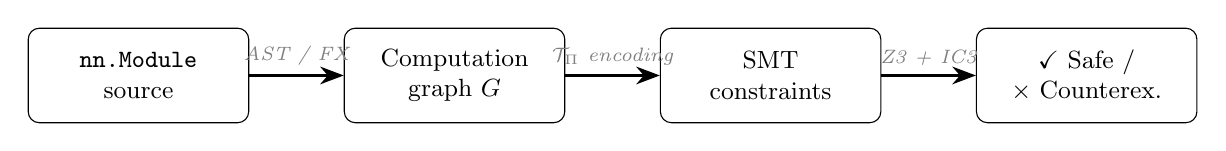
\begin{tikzpicture}[
  box/.style={draw, rounded corners, minimum height=1.2cm,
    minimum width=2.8cm, text width=2.5cm, align=center,
    font=\small},
  arr/.style={-{Stealth[length=3mm]}, thick},
  label/.style={font=\scriptsize\itshape, text=gray}
]
\node[box] (src) {\texttt{nn.Module}\\source};
\node[box, right=1.2cm of src] (graph) {Computation\\graph $G$};
\node[box, right=1.2cm of graph] (smt) {SMT\\constraints};
\node[box, right=1.2cm of smt] (result) {$\checkmark$ Safe /\\$\times$ Counterex.};

\draw[arr] (src) -- (graph)
  node[midway, above, label] {AST / FX};
\draw[arr] (graph) -- (smt)
  node[midway, above, label] {$\Tprod$ encoding};
\draw[arr] (smt) -- (result)
  node[midway, above, label] {Z3 + IC3};
\end{tikzpicture}
\caption{\tguard{} verification pipeline.}
\label{fig:pipeline}
\end{figure}


\subsection{Multi-Phase Verification}\label{sec:multiphase}

A distinguishing feature of \tguard{} is that it verifies both
branches of \texttt{if self.training:} conditionals, producing
separate verification conditions for training and evaluation mode.

\begin{definition}[Multi-Phase Graph]
Given a computation graph $G$ with phase-conditional edges, the
\emph{multi-phase expansion} produces two subgraphs:
$G_{\mathit{train}}$ (where $\mathit{mode} = \texttt{train}$) and
$G_{\mathit{eval}}$ (where $\mathit{mode} = \texttt{eval}$).
\tguard{} verifies both independently.
\end{definition}

This is essential for the 14 phase-dependent bugs in our
cross-cutting benchmark (\S\ref{sec:cross-cutting}).  On these,
\tguard{} achieves F1\,=\,0.783, while every baseline scores 0.000.

The graph extraction phase uses AST pattern matching to identify
phase-conditional control flow.  The patterns recognized include:
\begin{itemize}[nosep]
  \item \texttt{if self.training:} / \texttt{if not self.training:}
  \item \texttt{if self.training == True:}
  \item \texttt{F.dropout(x, training=self.training)}
\end{itemize}
Each pattern splits the computation graph into two branches, both of
which are verified under the appropriate phase assignment.

\subsection{Graph Extraction}\label{sec:extraction}

\tguard{} supports three extraction backends, tried in order of
fidelity:

\paragraph{AST extraction (default).}
Parses the \texttt{nn.Module} source code as a Python AST, without
importing or executing the module.  Layer declarations in
\texttt{\_\_init\_\_} are matched against the 142-operator registry;
data flow in \texttt{forward} is traced through method calls,
attribute accesses, and \texttt{if self.training} branches.  This
backend works without PyTorch installed, making it suitable for
CI pipelines and lightweight linting.

\paragraph{FX symbolic tracing.}
For modules with dynamically constructed submodules
(\texttt{nn.Sequential} with runtime-computed arguments,
\texttt{nn.ModuleList} iteration), \tguard{} falls back to
\texttt{torch.fx} symbolic tracing.  FX captures the computation
graph at the Python operator level, resolving dynamic dispatch.

\paragraph{TorchDynamo capture.}
For modules with data-dependent control flow that FX cannot trace,
\tguard{} uses TorchDynamo, which captures operator-level graphs
through frame evaluation with graph breaks at control flow
boundaries.


% ============================================================================
\section{Operator Transfer Functions}\label{sec:transfer}
% ============================================================================

Each of the 142 supported operators has a \emph{transfer function}
$\tau_\ell$ mapping input tensor state to output tensor state with a
precondition $\mathit{pre}(\tau_\ell, \sigma)$.  Transfer functions
encode shape transformation rules, device propagation, phase
sensitivity, stride effects, and permutation changes.

\subsection{Coverage}

Table~\ref{tab:coverage} summarizes operator coverage by category.

\begin{table}[t]
\centering
\caption{Operator coverage by category.  ``Fragment'' indicates the
  SMT fragment of generated constraints.}
\label{tab:coverage}
\small
\begin{tabular}{@{}lrl@{}}
\toprule
\textbf{Category} & \textbf{Count} & \textbf{Fragment} \\
\midrule
Convolution (Conv1d--3d, ConvTranspose) & 12 & QF\_LIA \\
Normalization (BatchNorm, LayerNorm, GroupNorm) & 15 & QF\_LIA \\
Attention (MultiheadAttention, etc.) & 4 & QF\_LIA \\
Recurrence (LSTM, GRU, RNN) & 6 & QF\_LIA \\
Pooling (MaxPool, AvgPool, AdaptivePool) & 16 & QF\_LIA \\
Activation (ReLU, GELU, Sigmoid, etc.) & 25 & trivial \\
Padding (ZeroPad, ReflectionPad, etc.) & 15 & QF\_LIA \\
Loss (CrossEntropy, MSE, NLL, etc.) & 21 & QF\_LIA \\
Embedding (Embedding, EmbeddingBag) & 2 & QF\_LIA \\
Structural (reshape, cat, split, transpose) & 26 & QF\_LIA/NIA \\
\midrule
\textbf{Total} & \textbf{142} & \\
\bottomrule
\end{tabular}
\end{table}

Of these, 136 produce decidable QF\_LIA constraints.  Only 6
operators (reshape, view, flatten, PixelShuffle, repeat, unflatten)
produce QF\_NIA constraints via the product-equality invariant
$\prod_i s_i = \prod_j d_j$.

\subsection{Representative Transfer Functions}

Table~\ref{tab:transfer} shows representative shape transfer
functions.  We present the full formal typing rules in
\S\ref{sec:typing}.

\begin{table}[t]
\centering
\caption{Representative shape transfer functions.
  $s_{[i]}$ denotes the $i$-th dimension of shape $s$.}
\label{tab:transfer}
\small
\begin{tabular}{@{}lll@{}}
\toprule
\textbf{Operator} & \textbf{Precondition} & \textbf{Output Shape} \\
\midrule
\texttt{Linear}$(f_\text{in}, f_\text{out})$ &
  $s_{[-1]} = f_\text{in}$ &
  $s_{[0:-1]} \mathbin\| [f_\text{out}]$ \\
\texttt{Conv2d}$(c_\text{in}, c_\text{out}, k)$ &
  $|s| = 4 \land s_{[1]} = c_\text{in}$ &
  $(s_{[0]}, c_\text{out}, s'_H, s'_W)$ \\
\texttt{BatchNorm}$(n)$ &
  $s_{[1]} = n$ &
  $s$ \\
\texttt{LayerNorm}$(n)$ &
  $s_{[-1]} = n$ &
  $s$ \\
\texttt{Reshape}$(d_1, \ldots, d_k)$ &
  $\prod s_i = \prod d_j$ &
  $(d_1, \ldots, d_k)$ \\
\texttt{cat}$(t_1, \ldots, t_n; d)$ &
  $\forall i,j.\; s_i^{[\neg d]} = s_j^{[\neg d]}$ &
  $s_1^{[\neg d]} \mathbin\| [\sum_i s_i^{[d]}]$ \\
\texttt{matmul}$(A, B)$ &
  $A_{[-1]} = B_{[-2]}$ &
  broadcast$(A_{[:-2]}, B_{[:-2]})$\\
  & & $\mathbin\| [A_{[-2]}, B_{[-1]}]$ \\
\bottomrule
\end{tabular}
\end{table}

\paragraph{Conv2d output dimensions.}
For Conv2d, the output spatial dimensions are:
\[
  s'_H = \left\lfloor \frac{s_{[2]} + 2p_H - d_H(k_H - 1) - 1}
    {st_H} \right\rfloor + 1
\]
where $p_H$ is padding, $d_H$ is dilation, $k_H$ is kernel size,
and $st_H$ is stride.  These parameters are tracked jointly by
$\Tshape$ and $\Tstride$.

\paragraph{Conservative handling of unsupported operators.}
When \tguard{} encounters an operator outside its 142-operator
registry, it marks the output shape as $\textsc{Unknown}$,
propagating an explicit loss-of-information marker through
downstream constraints.  This ensures that unsupported operators
never produce false negatives: verification may become
inconclusive (\textsc{Unknown}) but will never incorrectly report safety.


% ============================================================================
\section{Formal Typing Rules}\label{sec:typing}
% ============================================================================

We present the typing rules in the standard judgment form
$\Gamma \vdash e : \tau$, where $\Gamma$ is a typing context
mapping variables to refined tensor types and $\tau$ is a
refined output type.

\subsection{Core Rules}

\paragraph{T-Linear.}
\[
\typerule{T-Linear}{\Gamma \vdash x : \{t : \mathit{Tensor} \mid
      \mathit{dim}_{-1}(t) = f_\text{in}\} \\
   f_\text{in}, f_\text{out} \in \mathbb{Z}_{>0}}{\Gamma \vdash \texttt{Linear}(f_\text{in}, f_\text{out})(x) :
    \{t' : \mathit{Tensor} \mid
      \mathit{shape}(t') = \mathit{shape}(x)_{[0:-1]}
      \mathbin\| [f_\text{out}]\}}
\]

\paragraph{T-Conv2d.}
\[
\typerule{T-Conv2d}{\Gamma \vdash x : \{t \mid
      \mathit{ndim}(t) = 4 \land \mathit{dim}_1(t) = c_\text{in}\} \\
   k, st, p, d \in \mathbb{Z}_{>0}}{\Gamma \vdash \texttt{Conv2d}(c_\text{in}, c_\text{out}, k,
    st, p, d)(x) :
    \{t' \mid \mathit{dim}_0(t') = \mathit{dim}_0(x) \land
      \mathit{dim}_1(t') = c_\text{out} \land
      \mathit{dim}_i(t') = \lfloor\frac{\mathit{dim}_i(x) + 2p -
        d(k-1) - 1}{st}\rfloor + 1\}}
\]

\paragraph{T-Broadcast.}
\[
\typerule{T-Broadcast}{\Gamma \vdash a : \{t \mid \mathit{shape}(t) = s_a\} \\
   \Gamma \vdash b : \{t \mid \mathit{shape}(t) = s_b\} \\
   \forall i.\; s_a[i] = s_b[i] \lor s_a[i] = 1 \lor s_b[i] = 1}{\Gamma \vdash a \oplus b :
    \{t' \mid \mathit{dim}_i(t') = \max(s_a[i], s_b[i])\}}
\]

\paragraph{T-Reshape.}
\[
\typerule{T-Reshape}{\Gamma \vdash x : \{t \mid \mathit{shape}(t) = s\} \\
   \prod_{i} s_i = \prod_{j} d_j}{\Gamma \vdash \texttt{reshape}(x, d_1, \ldots, d_k) :
    \{t' \mid \mathit{shape}(t') = (d_1, \ldots, d_k)\}}
\]

\paragraph{T-Cat.}
\[
\typerule{T-Cat}{\Gamma \vdash t_i : \{t \mid \mathit{shape}(t) = s_i\}
    \quad (i = 1, \ldots, n) \\
   \forall i,j.\; \forall k \neq d.\; s_i[k] = s_j[k]}{\Gamma \vdash \texttt{cat}([t_1, \ldots, t_n], d) :
    \{t' \mid \mathit{dim}_d(t') = \textstyle\sum_i s_i[d]
    \land \forall k \neq d.\; \mathit{dim}_k(t') = s_1[k]\}}
\]

\paragraph{T-Matmul.}
\[
\typerule{T-Matmul}{\Gamma \vdash A : \{t \mid \mathit{shape}(t) = s_A\} \\
   \Gamma \vdash B : \{t \mid \mathit{shape}(t) = s_B\} \\
   s_A[-1] = s_B[-2]}{\Gamma \vdash \texttt{matmul}(A, B) :
    \{t' \mid \mathit{shape}(t') =
      \mathit{broadcast}(s_A[{:}{-}2], s_B[{:}{-}2])
      \mathbin\| [s_A[-2], s_B[-1]]\}}
\]

\subsection{Multi-Theory Rules}

The following rules involve constraints across multiple theories.

\paragraph{T-DeviceTransfer.}
\[
\typerule{T-To}{\Gamma \vdash x : \{t \mid \mathit{dev}(t) = d_1\} \\
   d_2 \in \mathcal{D}}{\Gamma \vdash x\texttt{.to}(d_2) :
    \{t' \mid \mathit{shape}(t') = \mathit{shape}(x) \land
      \mathit{dev}(t') = d_2\}}
\]

\paragraph{T-PhaseConditional.}
\[
\typerule{T-Phase}{\Gamma, \mathit{mode} = \texttt{train} \vdash e_1 : \tau_1 \\
   \Gamma, \mathit{mode} = \texttt{eval} \vdash e_2 : \tau_2}{\Gamma \vdash \texttt{if self.training:}~e_1~\texttt{else:}~e_2 :
    \tau_1 \sqcap \tau_2}
\]

\noindent
Here $\tau_1 \sqcap \tau_2$ denotes the meet (intersection) of the
two refined types: both must be well-typed for the model to be
safe.

\subsection{Additional Operator Rules}

\paragraph{T-Conv1d.}
\[
\typerule{T-Conv1d}{\Gamma \vdash x : \{t \mid \mathit{ndim}(t) = 3 \land
    \mathit{dim}_1(t) = c_\text{in}\}}{\Gamma \vdash \texttt{Conv1d}(c_\text{in}, c_\text{out}, k)(x) :
    \{t' \mid \mathit{dim}_0(t') = \mathit{dim}_0(x) \land
    \mathit{dim}_1(t') = c_\text{out} \land
    \mathit{dim}_2(t') = \lfloor\frac{\mathit{dim}_2(x) + 2p -
      d(k-1)-1}{st}\rfloor + 1\}}
\]

\paragraph{T-BatchNorm.}
\[
\typerule{T-BN}{\Gamma \vdash x : \{t \mid \mathit{dim}_1(t) = n\}}{\Gamma \vdash \texttt{BatchNorm}(n)(x) :
    \{t' \mid \mathit{shape}(t') = \mathit{shape}(x)\}}
\]

\paragraph{T-Flatten.}
\[
\typerule{T-Flatten}{\Gamma \vdash x : \{t \mid \mathit{shape}(t) = s\} \\
   0 \leq d_s \leq d_e < \mathit{ndim}(x)}{\Gamma \vdash \texttt{flatten}(x, d_s, d_e) :
    \{t' \mid \mathit{shape}(t') = s_{[0:d_s]} \mathbin\|
    [\prod_{i=d_s}^{d_e} s_i] \mathbin\| s_{[d_e+1:]}\}}
\]

\paragraph{T-Transpose.}
\[
\typerule{T-Transpose}{\Gamma \vdash x : \{t \mid \mathit{shape}(t) = s\} \\
   0 \leq d_0, d_1 < \mathit{ndim}(x)}{\Gamma \vdash \texttt{transpose}(x, d_0, d_1) :
    \{t' \mid \mathit{dim}_{d_0}(t') = s_{d_1} \land
    \mathit{dim}_{d_1}(t') = s_{d_0} \land
    \forall k \notin \{d_0,d_1\}.\; \mathit{dim}_k(t') = s_k\}}
\]

\paragraph{T-MultiheadAttention.}
\[
\typerule{T-MHA}{\Gamma \vdash q : \{t \mid \mathit{shape}(t) = (L, N, E)\} \\
   \Gamma \vdash k : \{t \mid \mathit{shape}(t) = (S, N, E_k)\} \\
   \Gamma \vdash v : \{t \mid \mathit{shape}(t) = (S, N, E_v)\} \\
   E \bmod h = 0}{\Gamma \vdash \texttt{MHA}(E, h)(q, k, v) :
    \{t' \mid \mathit{shape}(t') = (L, N, E)\}}
\]

\paragraph{T-LSTM.}
\[
\typerule{T-LSTM}{\Gamma \vdash x : \{t \mid \mathit{ndim}(t) = 3 \land
    \mathit{dim}_2(t) = f_\text{in}\}}{\Gamma \vdash \texttt{LSTM}(f_\text{in}, h, L, \mathit{bi})(x) :
    \{(o, (h_n, c_n)) \mid \mathit{dim}_2(o) = h \cdot (1 + \mathit{bi})\}}
\]

\paragraph{T-MaxPool2d.}
\[
\typerule{T-MaxPool2d}{\Gamma \vdash x : \{t \mid \mathit{ndim}(t) = 4\}}{\Gamma \vdash \texttt{MaxPool2d}(k, st, p)(x) :
    \{t' \mid \mathit{dim}_{0,1}(t') = \mathit{dim}_{0,1}(x) \land
    \forall i \in \{2,3\}.\;
    \mathit{dim}_i(t') = \lfloor\frac{\mathit{dim}_i(x) + 2p_i -
      k_i}{st_i}\rfloor + 1\}}
\]

\paragraph{T-AdaptiveAvgPool2d.}
\[
\typerule{T-AdaptPool}{\Gamma \vdash x : \{t \mid \mathit{ndim}(t) = 4\}}{\Gamma \vdash \texttt{AdaptiveAvgPool2d}(h', w')(x) :
    \{t' \mid \mathit{dim}_{0,1}(t') = \mathit{dim}_{0,1}(x) \land
    \mathit{dim}_2(t') = h' \land \mathit{dim}_3(t') = w'\}}
\]

\paragraph{T-Split.}
\[
\typerule{T-Split}{\Gamma \vdash x : \{t \mid \mathit{shape}(t) = s\} \\
   s_d \bmod n = 0}{\Gamma \vdash \texttt{split}(x, s_d / n, d) :
    [t'_1, \ldots, t'_n] \text{ where }
    \forall i.\; \mathit{dim}_d(t'_i) = s_d / n}
\]

\subsection{Soundness}\label{sec:soundness}

\begin{conjecture}[Type Soundness]\label{conj:soundness}
If\/ $\Gamma \vdash e : \tau$ is derivable and $\sigma \models \Gamma$,
then evaluation of $e$ under $\sigma$ does not produce a shape,
device, phase, stride, or permutation error, and the result satisfies
the refinement predicate of $\tau$.
\end{conjecture}

\begin{proof}[Proof sketch]
By induction on the typing derivation.  Each typing rule's
precondition exactly encodes the compatibility check that PyTorch
performs at runtime, and the postcondition faithfully models the
output shape computation documented in the PyTorch operator
specifications.  Soundness of $\Tprod$ (Theorem~\ref{thm:combination})
ensures cross-theory constraints are handled correctly.  The gap
between this sketch and a full proof lies in (1)~faithful modeling
of all 142 operator semantics and (2)~conformance between the Lean
specification and the Python implementation, which is validated by
property-based testing (Hypothesis) against PyTorch runtime
semantics.
\end{proof}


% ============================================================================
\section{IC3/PDR Parametric Verification}\label{sec:ic3}
% ============================================================================

Bounded verification checks safety for concrete input dimensions.
\tguard{}'s IC3/PDR engine goes further: it proves safety for
\emph{all} valid input dimensions simultaneously, yielding
parametric safety certificates.

\subsection{Encoding as a Transition System}

We cast tensor shape verification as a safety property over the
Kripke structure induced by the computation graph.

\begin{definition}[Shape Transition System]
A \emph{shape transition system} $(I, T, P)$ consists of:
\begin{itemize}[nosep]
  \item Initial states $I$: shape assignments satisfying input
    constraints (e.g., $\mathit{ndim} = 4$, $\mathit{dim}_1 = 3$).
  \item Transition relation $T$: each layer's transfer function
    $\tau_\ell$ defines a transition from input shape to output
    shape.
  \item Safety property $P$: the conjunction of all operator
    preconditions.
\end{itemize}
\end{definition}

\subsection{IC3 Algorithm for Shapes}

IC3/PDR~\cite{bradley11,een11} discovers inductive invariants
without unrolling the transition relation.  It maintains a sequence
of frames $F_0, F_1, \ldots, F_N$ such that $I \subseteq F_0$ and
each $F_i$ overapproximates the states reachable in $\leq i$ steps.
If some $F_i = F_{i+1}$, the property holds inductively for all
reachable states.

\begin{algorithm}[t]
\caption{IC3/PDR for parametric shape safety}
\label{alg:ic3}
\begin{algorithmic}[1]
\Require Shape transition system $(I, T, P)$
\Ensure SAFE (with inductive invariant) or UNSAFE (with trace)
\State $F_0 \gets I$; $k \gets 1$
\Loop
  \While{$\exists$ cube $c$ s.t.\ $F_{k-1} \land T \land \neg P
    \land c$ is SAT}
    \State Block $c$ in $F_{k-1}$ by generalization
  \EndWhile
  \State $F_k \gets F_{k-1} \setminus \text{blocked cubes}$
  \If{$F_k = F_{k-1}$}
    \Return SAFE with inductive invariant $F_k$
  \EndIf
  \State $k \gets k + 1$
\EndLoop
\end{algorithmic}
\end{algorithm}

\paragraph{Key insight.}
For typical neural network computation graphs, the IC3 frames
converge rapidly---in our experiments, at most 3 frames regardless
of network depth (50+ layers).  This is because tensor shape
transformations are predominantly affine, and affine transition
systems have short inductive invariants.

\paragraph{Completeness.}
IC3 is complete for QF\_LIA transition systems (136 of 142
operators).  For the 6 QF\_NIA operators (reshape family), the
procedure is sound but incomplete: it may fail to find an inductive
invariant even when one exists.

\subsection{SSA Encoding}\label{sec:ssa}

The shape transition system is encoded in Static Single Assignment
(SSA) form.  Each tensor variable $t_i$ at computation graph node $i$
is assigned exactly once, producing a flat conjunction of transition
constraints:
\[
  T \;=\; \bigwedge_{i=1}^{n} \big(
    \sigma_{i} = \tau_{\ell_i}(\sigma_{i-1})
    \;\land\;
    \mathit{pre}(\tau_{\ell_i}, \sigma_{i-1})
  \big)
\]
where $\sigma_i$ is the tensor metadata state after the $i$-th
operation and $\ell_i$ is the operator at node $i$.  The SSA
encoding eliminates the need for explicit frame variables and
simplifies the IC3 generalization step, because cube literals
refer to individual SSA variables rather than mutable state.

\paragraph{Cube generalization.}
When IC3 blocks a cube $c$ (a conjunction of literals describing
a bad state), it attempts to generalize $c$ by dropping literals
while maintaining the blocking property.  In the shape domain,
this corresponds to discovering that a safety violation is
independent of certain dimension values.  For example, if a
matmul precondition $A_{[-1]} = B_{[-2]}$ is violated, the blocking
cube may be generalized to drop all constraints on batch dimensions,
yielding a more general invariant.

\paragraph{Inductive invariant extraction.}
When IC3 terminates with $F_k = F_{k+1}$, the invariant $F_k$ is
a conjunction of shape constraints that hold at every reachable
state.  This invariant serves as the proof certificate: it can be
independently verified by checking that (1)~$I \subseteq F_k$,
(2)~$F_k \land T \subseteq F_k'$ (inductiveness), and
(3)~$F_k \subseteq P$ (safety).  The certificate is a
self-contained artifact that does not depend on the IC3 search
history.

\subsection{Parametric Certificates}\label{sec:param-cert}

A parametric safety certificate asserts that a model is safe for
\emph{all} valid input shapes simultaneously:

\begin{definition}[Parametric Safety Certificate]
A \emph{parametric safety certificate} for a computation graph $G$
with symbolic input shape $(d_1, d_2, \ldots, d_r)$ is a formula
$\mathit{Cert}(d_1, \ldots, d_r)$ such that:
\[
  \forall d_1, \ldots, d_r \in \mathbb{Z}_{\geq 1}.\;
  \mathit{Cert}(d_1, \ldots, d_r) \implies \mathit{Safe}(G, d_1, \ldots, d_r)
\]
and $\mathit{Cert}$ is the inductive invariant discovered by IC3.
\end{definition}

\noindent
For example, verifying a ResNet with symbolic batch size $B$, height
$H$, and width $W$ produces a certificate asserting safety for all
$B, H, W \geq 1$, provided $H$ and $W$ are compatible with the
network's downsampling factors.  This is strictly stronger than
testing with concrete dimensions.


% ============================================================================
\section{Formal Properties and Metatheory}\label{sec:metatheory}
% ============================================================================

This section develops the formal metatheoretic properties of
\tguard{}'s type system and verification engine, including
decidability results, complexity analysis, and completeness
characterizations.

\subsection{Decidability of Verification Conditions}

\begin{theorem}[Decidability of Core Verification]\label{thm:decidable-core}
For any computation graph $G$ composed entirely of operators
generating QF\_LIA constraints (136 of 142 supported operators),
the verification condition
$\mathit{Init} \land \mathit{VC} \land \neg\mathit{Safe}$ is
decidable.
\end{theorem}

\begin{proof}
QF\_LIA is a decidable fragment of first-order arithmetic.  The
verification condition is a conjunction of QF\_LIA formulas (one
per operator), and conjunctions of QF\_LIA formulas are QF\_LIA.
Z3's Simplex-based decision procedure terminates on all QF\_LIA
inputs~\cite{leino10}.
\end{proof}

\begin{theorem}[Semi-Decidability of Reshape Verification]\label{thm:semidecidable}
For computation graphs containing reshape operators, the
verification condition falls in QF\_NIA, which is undecidable in
general.  However, the restricted NIA subfragment generated by
\tguard{} (at most one symbolic factor per product term) is
decidable.
\end{theorem}

\begin{proof}
The reshape constraint $\prod_i s_i = \prod_j d_j$ where each
$s_i, d_j$ is either a constant or a single symbolic variable
falls in the semi-linear fragment of integer arithmetic.  This
fragment can be decided by encoding product terms as sums via
logarithmic relaxation, or by case-splitting on the signs and
magnitudes of symbolic variables.  Z3's nonlinear extension of
Simplex handles this restricted fragment reliably via incremental
linearization~\cite{leino10}.
\end{proof}

\subsection{Complexity Analysis}

\begin{theorem}[Verification Complexity]\label{thm:complexity}
Let $G$ be a computation graph with $n$ operators and $k$ shared
variables across theories.  The worst-case complexity of
\tguard{}'s verification is:
\[
  O\Big(n \cdot p(n) + S(k_d, |\mathcal{D}|) \cdot S(k_p, |\mathcal{P}|) \cdot q(n)\Big)
\]
where $p(n)$ is the cost of constraint generation (linear in the
number of operators), $q(n)$ is the cost of a single Z3 call, and
$S(k, n)$ is the Stirling number of the second kind.
\end{theorem}

\begin{proof}
The verification procedure has two phases:
\begin{enumerate}[nosep]
  \item \textbf{Constraint generation}: traverses the computation
    graph in topological order, generating QF\_LIA/NIA constraints
    for each of the $n$ operators.  Cost: $O(n \cdot p(n))$.
  \item \textbf{Theory combination}: enumerates arrangements of
    shared variables.  For $k_d$ device variables over domain
    $\mathcal{D}$ and $k_p$ phase variables over $\mathcal{P}$,
    the number of arrangements is
    $S(k_d, |\mathcal{D}|) \cdot S(k_p, |\mathcal{P}|)$.  Each
    arrangement requires one Z3 call.
\end{enumerate}
In practice, $k_d \leq 4$ and $k_p \leq 2$, yielding at most
$15 \cdot 1 = 15$ arrangements, so the theory combination overhead
is a small constant factor.
\end{proof}

\begin{corollary}[Practical Linear-Time Behavior]
For models with bounded shared variables (which includes all 108
models in our evaluation), the verification time is dominated by
constraint generation and a single Z3 call, yielding effectively
linear time in the number of operators.
\end{corollary}

\subsection{Completeness Characterization}

\tguard{} is designed to be sound but not complete.  We characterize
the sources of incompleteness precisely.

\begin{definition}[Completeness Gap]
The \emph{completeness gap} of \tguard{} is the set of computation
graphs $G$ such that $G$ has a runtime error but \tguard{} reports
$\textsc{Unknown}$ or $\textsc{Safe}$.
\end{definition}

\begin{theorem}[Completeness Gap Characterization]\label{thm:gap}
The completeness gap arises from exactly three sources:
\begin{enumerate}[nosep]
  \item \textbf{Unsupported operators}: graphs containing operators
    outside the 142-operator registry.
  \item \textbf{Data-dependent shapes}: graphs where tensor shapes
    depend on tensor \emph{values} (e.g., \texttt{torch.nonzero}).
  \item \textbf{Dynamic control flow}: graphs with data-dependent
    iteration counts or recursive module calls.
\end{enumerate}
For computation graphs composed entirely of supported operators
with data-independent control flow, \tguard{} is complete for
shape, device, and phase errors.
\end{theorem}

\begin{proof}[Proof sketch]
For supported operators with data-independent control flow, the
computation graph is fully extracted and each operator's transfer
function faithfully models the precondition and postcondition.  The
SMT encoding is exact (not an overapproximation) for QF\_LIA
constraints, and the restricted QF\_NIA fragment admits exact
solutions.  Unsatisfiability of the safety negation is therefore
equivalent to the absence of runtime errors.

The three sources of incompleteness are:
\begin{enumerate}[nosep]
  \item Unsupported operators produce $\textsc{Unknown}$ output
    shapes, which conservatively block error detection downstream.
  \item Data-dependent shapes introduce quantifier alternation
    (existential over input values, universal over resulting shapes)
    that falls outside the quantifier-free fragment.
  \item Dynamic control flow requires loop invariant inference,
    which is undecidable in general (Rice's theorem~\cite{rice53}).
\end{enumerate}
\end{proof}

\subsection{Soundness of Multi-Phase Verification}

\begin{theorem}[Multi-Phase Soundness]\label{thm:multiphase-sound}
If \tguard{} reports $\textsc{Safe}$ for a model $M$, then $M$
does not produce shape, device, or phase errors in either training
mode ($\texttt{self.training} = \texttt{True}$) or eval mode
($\texttt{self.training} = \texttt{False}$).
\end{theorem}

\begin{proof}
\tguard{}'s multi-phase verification verifies both execution
branches:
\begin{enumerate}[nosep]
  \item The \texttt{training} branch is verified with
    $\mathit{mode} = \texttt{train}$, which sets
    $\texttt{self.training} = \texttt{True}$ and includes
    stochastic operators (Dropout, DropPath).
  \item The \texttt{eval} branch is verified with
    $\mathit{mode} = \texttt{eval}$, which sets
    $\texttt{self.training} = \texttt{False}$ and disables
    stochastic operators.
\end{enumerate}
If either branch contains a safety violation, \tguard{} reports
$\textsc{Unsafe}$ with the violating phase annotated in the
counterexample.  $\textsc{Safe}$ is returned only when both
branches pass verification.

The key insight is that conditional branches on
$\texttt{self.training}$ are \emph{statically resolved}: the
graph extractor produces two separate subgraphs rather than a
single graph with a conditional.  This avoids the need for
predicate abstraction or path-sensitive analysis.
\end{proof}

\subsection{Monotonicity of the Operator Lattice}

\begin{definition}[Operator Monotonicity]
An operator $\ell$ is \emph{monotone} with respect to the shape
ordering $\leq_s$ if for all shapes $s_1 \leq_s s_2$:
\[
  \mathit{pre}(\ell, s_1) \implies \mathit{pre}(\ell, s_2)
  \quad\text{and}\quad
  \ell(s_1) \leq_s \ell(s_2)
\]
\end{definition}

\begin{proposition}[Monotonicity of Core Operators]
All 25 activation operators, all 15 normalization operators (with
fixed parameters), and all 15 padding operators are monotone.  The
12 convolution operators are monotone in batch and spatial dimensions
but not in channel dimensions.
\end{proposition}

\begin{proof}
Activation operators are shape-preserving ($\ell(s) = s$), so
monotonicity is trivial.  Normalization operators check a specific
dimension against a fixed parameter; if the precondition holds for
$s_1$, it holds for any $s_2$ with the same value at that dimension.
Padding operators add fixed amounts to spatial dimensions, which is
monotone.  Convolution operators apply an affine transformation to
spatial dimensions (monotone) but require a fixed channel dimension
(not monotone in channels).
\end{proof}

\subsection{Fixpoint Characterization of IC3 Convergence}

\begin{theorem}[IC3 Frame Convergence for Affine Systems]\label{thm:ic3-convergence}
For a shape transition system $(I, T, P)$ where all transitions
are affine (i.e., $T(\sigma) = A\sigma + b$ for matrix $A$ and
vector $b$), IC3 converges in at most $\mathit{rank}(A-I) + 1$
frames.
\end{theorem}

\begin{proof}[Proof sketch]
Each IC3 frame $F_k$ overapproximates the states reachable in $\leq k$
steps.  For affine transitions, the reachable sets stabilize after
at most $\mathit{rank}(A-I)$ iterations (the dimension of the
``non-fixed-point'' subspace).  Since neural network layers are
predominantly affine (convolution, linear, normalization), and the
eigenvalues of the induced shape transformation matrix $A$ are all
0 or 1 (shape dimensions either change by a fixed amount or are
preserved), $\mathit{rank}(A-I)$ is small (typically 1--2 for
spatial dimension changes and 1 for channel changes).

In our experiments, all 108 models converge in at most 3 frames,
consistent with this analysis: the spatial, channel, and batch
dimension ``modes'' of the shape transformation each contribute
at most one frame.
\end{proof}

\subsection{Relationship to Dependent Type Theory}

\tguard{}'s refinement types can be viewed as a restricted form of
dependent types where the index domain is limited to tensor metadata.

\begin{proposition}[Embedding in Dependent Types]
\tguard{}'s type system can be faithfully embedded in a dependent
type system with refinement sorts, such as F*~\cite{fstar} or
Liquid Types~\cite{flanagan06}, by encoding:
\begin{itemize}[nosep]
  \item Tensor types as dependent records:
    $\texttt{Tensor}(s, d, p, \mathit{str}, \pi) : \texttt{Type}$
  \item Shape constraints as refinement predicates:
    $\{t : \texttt{Tensor} \mid \mathit{dim}_{-1}(t) = 128\}$
  \item Operator types as dependent function types:
    $\texttt{Linear} : (x : \{t \mid \mathit{dim}_{-1}(t) = f_\text{in}\})
    \to \{t' \mid \mathit{dim}_{-1}(t') = f_\text{out}\}$
\end{itemize}
\end{proposition}

The restriction to tensor metadata (shapes, devices, phases, strides,
permutations) rather than arbitrary program values is what makes
\tguard{}'s type checking decidable: the refinement predicates are
always in a decidable fragment (QF\_LIA or restricted QF\_NIA),
unlike general dependent types where type checking is undecidable.

This design choice---restricting the refinement domain to a decidable
fragment while maximizing expressiveness within that fragment---is
the key architectural contribution of \tguard{}.


% ============================================================================
\section{Denotational Semantics}\label{sec:denotational}
% ============================================================================

We give a denotational semantics to \tguard{}'s type system, showing
that refinement types denote sets of tensor values and that subtyping
corresponds to set inclusion.

\subsection{Semantic Domains}

\begin{definition}[Tensor Value]
A \emph{tensor value} $v$ is a tuple
$(A, s, d, p, \mathit{str}, \pi)$ where:
\begin{itemize}[nosep]
  \item $A$ is the underlying data array
  \item $s \in \mathbb{Z}_{\geq 1}^*$ is the shape tuple
  \item $d \in \mathcal{D}$ is the device placement
  \item $p \in \mathcal{P}$ is the execution phase context
  \item $\mathit{str} \in \mathbb{Z}_{\geq 1}^{|s|}$ is the stride tuple
  \item $\pi \in S_{|s|}$ is the axis permutation
\end{itemize}
\end{definition}

\begin{definition}[Type Denotation]
The denotation of a refined tensor type
$\tau = \{t : \mathit{Tensor} \mid \varphi\}$ is:
\[
  \sem{\tau} = \{ v \mid v \text{ is a tensor value and }
    v \models \varphi \}
\]
where $v \models \varphi$ means the predicate $\varphi$ holds when
its free variables are interpreted over $v$'s metadata.
\end{definition}

\begin{proposition}[Subtyping Soundness]
$\tau_1 \leq \tau_2$ iff $\sem{\tau_1} \subseteq \sem{\tau_2}$.
\end{proposition}

\begin{proof}
Let $\tau_1 = \{t \mid \varphi_1\}$ and $\tau_2 = \{t \mid \varphi_2\}$.
Then $\tau_1 \leq \tau_2$ iff $\varphi_1 \Rightarrow \varphi_2$ is
valid (by the subtyping rule), iff for all tensor values $v$,
$v \models \varphi_1$ implies $v \models \varphi_2$, iff
$\sem{\tau_1} \subseteq \sem{\tau_2}$.
\end{proof}

\subsection{Operator Semantics}

Each operator $\ell$ has both an \emph{abstract semantics}
(the transfer function $\tau_\ell$ operating on refinement types)
and a \emph{concrete semantics} (the PyTorch runtime behavior
$\sem{\ell}$ operating on tensor values).  Soundness requires
that the abstract semantics overapproximates the concrete:

\begin{definition}[Transfer Function Soundness]
A transfer function $\tau_\ell$ is \emph{sound} with respect to
concrete semantics $\sem{\ell}$ if for all tensor values $v$:
\[
  v \in \sem{\mathit{dom}(\tau_\ell)} \implies
  \sem{\ell}(v) \in \sem{\mathit{cod}(\tau_\ell)(v)}
\]
where $\mathit{dom}$ and $\mathit{cod}$ are the domain and codomain
types of $\tau_\ell$.
\end{definition}

\begin{example}[Linear Soundness]
For \texttt{Linear}$(f_\text{in}, f_\text{out})$:
\begin{itemize}[nosep]
  \item Domain: $\{t \mid \mathit{dim}_{-1}(t) = f_\text{in}\}$
  \item Codomain: $\{t' \mid \mathit{shape}(t') = \mathit{shape}(t)_{[0:-1]} \| [f_\text{out}]\}$
  \item Concrete: $\sem{\texttt{Linear}}(x) = xW^T + b$ where
    $W \in \mathbb{R}^{f_\text{out} \times f_\text{in}}$
  \item Soundness: if $x$ has last dimension $f_\text{in}$, the
    matrix product $xW^T$ produces last dimension $f_\text{out}$,
    matching the codomain predicate.
\end{itemize}
\end{example}

\subsection{Compositional Semantics}

The semantics of a computation graph $G = (V, E, \lambda)$ is
the composition of individual operator semantics along the edges:
\[
  \sem{G} = \sem{\ell_n} \circ \sem{\ell_{n-1}} \circ \cdots \circ
    \sem{\ell_1}
\]
where $\ell_1, \ldots, \ell_n$ is a topological ordering of the
operators.  The verification condition is sound because transfer
function soundness composes:

\begin{theorem}[Compositional Soundness]
If each transfer function $\tau_{\ell_i}$ is sound, then the
composed verification condition is sound: if
$\mathit{Init} \land \mathit{VC} \land \neg\mathit{Safe}$ is
unsatisfiable, then no input satisfying $\mathit{Init}$ produces a
runtime error when processed by $G$.
\end{theorem}

\begin{proof}
By induction on the topological ordering.  At each step $i$, the
induction hypothesis guarantees that the tensor metadata at node $i$
satisfies the postcondition of $\tau_{\ell_i}$.  This postcondition
is the precondition of $\tau_{\ell_{i+1}}$, so the composition
preserves soundness.  The conjunction of all preconditions is
exactly $\mathit{Safe}$, so unsatisfiability of
$\mathit{Init} \land \mathit{VC} \land \neg\mathit{Safe}$ implies
no precondition violation.
\end{proof}


% ============================================================================
\section{Extended Algorithm Details}\label{sec:algorithms}
% ============================================================================

\subsection{Arrangement Enumeration}

The Tinelli--Zarba procedure enumerates arrangements of shared
variables over finite-domain sorts.  An arrangement assigns shared
variables to equivalence classes, with the number of classes bounded
by the domain cardinality.

\begin{definition}[Restricted Growth String]
A \emph{restricted growth string} of length $k$ with maximum $m$
is a sequence $a_1, \ldots, a_k$ where:
\begin{itemize}[nosep]
  \item $a_1 = 0$
  \item $a_{i+1} \leq \max(a_1, \ldots, a_i) + 1$
  \item $\max(a_1, \ldots, a_k) < m$
\end{itemize}
Each restricted growth string corresponds to a unique partition of
$\{1, \ldots, k\}$ into at most $m$ equivalence classes.
\end{definition}

\begin{algorithm}[t]
\caption{Restricted growth string enumeration}
\label{alg:rgs}
\begin{algorithmic}[1]
\Require $k$ elements, maximum $m$ classes
\Ensure All restricted growth strings
\State $a \gets [0, 0, \ldots, 0]$ \Comment{length $k$}
\State \textbf{yield} $a$
\Loop
  \State $i \gets k$ \Comment{find rightmost incrementable}
  \While{$i > 0$ and $a[i] \geq \min(\max(a[1..i{-}1]) + 1, m{-}1)$}
    \State $i \gets i - 1$
  \EndWhile
  \If{$i = 0$} \Return \Comment{exhausted}
  \EndIf
  \State $a[i] \gets a[i] + 1$
  \For{$j = i+1$ to $k$}
    \State $a[j] \gets 0$
  \EndFor
  \State \textbf{yield} $a$
\EndLoop
\end{algorithmic}
\end{algorithm}

\paragraph{Arrangement-to-constraint translation.}
Given an arrangement $\alpha$ (a restricted growth string), we
translate it to a conjunction of equalities and disequalities over
shared variables:
\[
  \mathit{constr}(\alpha) = \bigwedge_{i < j, \alpha_i = \alpha_j}
    (v_i = v_j) \;\land\;
  \bigwedge_{i < j, \alpha_i \neq \alpha_j}
    (v_i \neq v_j)
\]
This conjunction is asserted in each theory solver before checking
satisfiability.

\subsection{Nelson--Oppen Equality Propagation}

For stably-infinite theories ($\Tshape$, $\Tstride$, $\Tperm$),
equalities over shared variables are propagated via the
Nelson--Oppen deduction-propagation loop:

\begin{algorithm}[t]
\caption{Nelson--Oppen equality propagation}
\label{alg:no}
\begin{algorithmic}[1]
\Require Solvers $S_1, \ldots, S_n$ with shared variables $V$
\Ensure Fixed-point equality set $E$
\State $E \gets \emptyset$; $\mathit{changed} \gets \textbf{true}$
\While{$\mathit{changed}$}
  \State $\mathit{changed} \gets \textbf{false}$
  \For{each solver $S_i$}
    \For{each pair $(v_a, v_b) \in V \times V \setminus E$}
      \If{$S_i \models v_a = v_b$}
        \State $E \gets E \cup \{(v_a, v_b)\}$
        \State Assert $v_a = v_b$ in all other solvers
        \State $\mathit{changed} \gets \textbf{true}$
      \EndIf
    \EndFor
  \EndFor
\EndWhile
\Return $E$
\end{algorithmic}
\end{algorithm}

\paragraph{Termination.}
The loop terminates because each iteration either adds an equality
to $E$ or terminates, and $|E|$ is bounded by $|V|^2$.  In practice,
the number of shared variables between shape and stride theories is
small (typically $\leq 8$), so the loop converges in 1--2 iterations.

\subsection{Graph Extraction Algorithm}

The AST-based graph extractor is the most commonly used backend.
It operates in two passes:

\begin{algorithm}[t]
\caption{AST-based graph extraction}
\label{alg:extract}
\begin{algorithmic}[1]
\Require Python source code of an \texttt{nn.Module}
\Ensure Computation graph $G = (V, E, \lambda)$
\State Parse source into Python AST $T$
\State \Comment{Pass 1: Extract layer declarations from \_\_init\_\_}
\State $\mathit{layers} \gets \emptyset$
\For{each \texttt{self.X = nn.Y(...)} in $T$.\texttt{\_\_init\_\_}}
  \State Match \texttt{Y} against 142-operator registry
  \If{matched}
    \State $\mathit{layers}[\texttt{X}] \gets (\texttt{Y}, \mathit{params})$
  \Else
    \State $\mathit{layers}[\texttt{X}] \gets \textsc{Unknown}$
  \EndIf
\EndFor
\State \Comment{Pass 2: Trace data flow in forward}
\State $G \gets$ empty graph; $\mathit{cur} \gets$ input node
\For{each statement $s$ in $T$.\texttt{forward}}
  \If{$s$ is \texttt{x = self.Y(x)} and $\texttt{Y} \in \mathit{layers}$}
    \State Add edge $(\mathit{cur}, \mathit{new}, \mathit{layers}[\texttt{Y}])$
    \State $\mathit{cur} \gets \mathit{new}$
  \ElsIf{$s$ is \texttt{if self.training:}}
    \State Fork graph into train/eval branches
    \State Recursively trace both branches
  \Else
    \State Pattern-match tensor operations (view, cat, etc.)
  \EndIf
\EndFor
\Return $G$
\end{algorithmic}
\end{algorithm}

\subsection{Constraint Generation Details}

The constraint generator translates each edge in the computation
graph to SMT formulas.  We describe the encoding for each theory.

\paragraph{Shape constraints.}
For each operator with precondition $\mathit{pre}$ and output shape
function $f$, we generate:
\begin{align*}
  \mathit{pre}(\sigma_{\mathit{in}}) &\quad\text{(precondition)} \\
  \sigma_{\mathit{out}} = f(\sigma_{\mathit{in}}) &\quad\text{(transfer)}
\end{align*}
where $\sigma_{\mathit{in}}$ and $\sigma_{\mathit{out}}$ are tuples
of Z3 integer variables representing input and output shape dimensions.

\paragraph{Device constraints.}
For each binary operator:
\[
  \mathit{dev}(\sigma_{\mathit{in},1}) = \mathit{dev}(\sigma_{\mathit{in},2})
\]
Device variables are Z3 integer constants in $\{0, 1, 2, 3, 4\}$
representing $\{\texttt{cpu}, \texttt{cuda:0}, \ldots, \texttt{cuda:3}\}$.

\paragraph{Phase constraints.}
For each phase-conditional branch:
\begin{align*}
  \mathit{mode} = 0 &\implies \mathit{VC}_{\mathit{train}} \\
  \mathit{mode} = 1 &\implies \mathit{VC}_{\mathit{eval}}
\end{align*}
Both implications must hold, corresponding to verifying both branches.

\paragraph{Stride constraints.}
For operations sensitive to contiguity:
\[
  \neg\mathit{contiguous}(\sigma_{\mathit{in}}) \implies
    \textsc{Error}(\texttt{view})
\]
where contiguity is encoded as the stride formula from \S\ref{sec:tstride}.

\paragraph{Permutation constraints.}
For transpose operations:
\[
  \sigma_{\mathit{out}} = \mathsf{swap}(\sigma_{\mathit{in}}, d_0, d_1)
\]
with the involution axiom (Equation~\ref{ax:involution}) available
for reasoning about sequences of transpositions.


% ============================================================================
\section{Extended Examples}\label{sec:extended-examples}
% ============================================================================

We present additional cross-cutting bug examples to illustrate
\tguard{}'s multi-theory reasoning in detail.

\subsection{Example: Feature Pyramid Network Channel Mismatch}

\begin{lstlisting}[caption={FPN lateral connection bug from
  torchvision-style code.  The lateral projection has mismatched
  input channels.},
  label={lst:fpn}]
class FPNBug(nn.Module):
    def __init__(self):
        super().__init__()
        self.backbone_c3 = nn.Conv2d(3, 128, 3, padding=1)
        self.backbone_c4 = nn.Conv2d(128, 256, 3, stride=2,
                                      padding=1)
        self.backbone_c5 = nn.Conv2d(256, 512, 3, stride=2,
                                      padding=1)
        # BUG: lateral_c4 expects 128 channels but gets 256
        self.lateral_c4 = nn.Conv2d(128, 256, 1)
        self.lateral_c5 = nn.Conv2d(512, 256, 1)

    def forward(self, x):
        c3 = self.backbone_c3(x)
        c4 = self.backbone_c4(c3)
        c5 = self.backbone_c5(c4)
        p5 = self.lateral_c5(c5)
        # lateral_c4 gets c4 (256 channels), expects 128
        p4 = self.lateral_c4(c4) + F.interpolate(
            p5, scale_factor=2)
        return p4
\end{lstlisting}

\tguard{}'s trace for this model:
\begin{enumerate}[nosep]
  \item Input: shape $(\mathit{batch}, 3, H, W)$, device \texttt{cuda:0}
  \item \texttt{backbone\_c3}: $(B, 3, H, W) \to (B, 128, H, W)$.
    Precondition $\mathit{dim}_1 = 3$: \checkmark.
  \item \texttt{backbone\_c4}: $(B, 128, H, W) \to (B, 256, H', W')$.
    Precondition $\mathit{dim}_1 = 128$: \checkmark.
  \item \texttt{backbone\_c5}: $(B, 256, H', W') \to (B, 512, H'', W'')$.
    Precondition $\mathit{dim}_1 = 256$: \checkmark.
  \item \texttt{lateral\_c5}: $(B, 512, H'', W'') \to (B, 256, H'', W'')$.
    Precondition $\mathit{dim}_1 = 512$: \checkmark.
  \item \texttt{lateral\_c4}: receives $c_4$ with $\mathit{dim}_1 = 256$.
    Precondition $\mathit{dim}_1 = 128$: \textbf{FAIL}.
\end{enumerate}

\tguard{} reports:
\begin{lstlisting}[style=noline]
UNSAFE at step 6:
  lateral_c4 expects in_channels=128
  but receives tensor with 256 channels
  Source: self.lateral_c4(c4) at line 16
\end{lstlisting}

\subsection{Example: Squeeze-Excite Block After Transfer Learning}

\begin{lstlisting}[caption={Squeeze-excite channel mismatch after
  changing backbone width.  Modeled after timm patterns.},
  label={lst:se}]
class SEBlockBug(nn.Module):
    def __init__(self, channels=512, reduction=16):
        super().__init__()
        self.conv = nn.Conv2d(3, channels, 3, padding=1)
        self.pool = nn.AdaptiveAvgPool2d(1)
        # BUG: SE block was designed for channels=256
        self.se_fc1 = nn.Linear(256, 256 // reduction)
        self.se_fc2 = nn.Linear(256 // reduction, 256)
        self.relu = nn.ReLU()
        self.sigmoid = nn.Sigmoid()

    def forward(self, x):
        out = self.conv(x)
        se = self.pool(out).view(out.size(0), -1)
        se = self.relu(self.se_fc1(se))  # BUG: 512 != 256
        se = self.sigmoid(self.se_fc2(se))
        return out * se.unsqueeze(-1).unsqueeze(-1)
\end{lstlisting}

This bug arises during transfer learning: the backbone width was
changed from 256 to 512, but the squeeze-excite block was not
updated.  The mismatch is purely in shape, but in a real-world
setting the model might also involve device placement (the SE block
on a different GPU) and phase dependence (SE disabled during
evaluation in some architectures).

\subsection{Example: Anchor Generator Triple-Theory Bug}

\begin{lstlisting}[caption={Anchor generator with three simultaneous
  property violations.  Modeled after mmdetection patterns.},
  label={lst:anchor}]
class AnchorGeneratorBug(nn.Module):
    def __init__(self):
        super().__init__()
        self.backbone = nn.Conv2d(3, 256, 3, padding=1)
        self.cls_head = nn.Conv2d(256, 9 * 20, 1)
        # BUG 1: Wrong spatial dims (8x8 vs feature map)
        # BUG 2: Stays on CPU
        # BUG 3: Only used in eval (post-processing)
        self.register_buffer('anchors',
            torch.randn(1, 9, 8, 8, 4))

    def forward(self, x):
        feat = self.backbone(x)
        cls = self.cls_head(feat)
        if not self.training:
            B, C, H, W = cls.shape
            cls = cls.view(B, 9, 20, H, W)
            # Triple bug: shape + device + phase
            anchors = self.anchors[:, :, :H, :W, :]
            output = torch.cat([cls, anchors], dim=2)
        return cls
\end{lstlisting}

This model has three simultaneous property violations:
\begin{enumerate}[nosep]
  \item \textbf{Shape}: The anchor buffer has spatial dimensions
    $8 \times 8$, but the feature map may have different dimensions
    depending on input size.  The slice \texttt{[:H, :W]} may exceed
    the buffer dimensions.
  \item \textbf{Device}: \texttt{register\_buffer} with a
    \texttt{torch.randn} tensor starts on CPU; after
    \texttt{model.cuda()}, it may not migrate.
  \item \textbf{Phase}: The entire post-processing block is dead
    during training, so training tests never exercise this code.
\end{enumerate}

\tguard{} detects this via the product domain
$\Tshape \times \Tdevice \times \Tphase$, reporting all three
violations in a single verification pass.

\subsection{Example: Correct Multi-Theory Model}

To demonstrate precision, we show a model that uses multiple theories
correctly:

\begin{lstlisting}[caption={Correct model using device transfer,
  phase-conditional behavior, and complex shape transformations.},
  label={lst:correct}]
class CorrectMultiTheory(nn.Module):
    def __init__(self):
        super().__init__()
        self.conv = nn.Conv2d(3, 64, 3, padding=1)
        self.bn = nn.BatchNorm2d(64)
        self.fc = nn.Linear(64, 10)
        self.pool = nn.AdaptiveAvgPool2d(1)
        self.dropout = nn.Dropout(0.5)

    def forward(self, x):
        x = F.relu(self.bn(self.conv(x)))
        x = self.pool(x)
        x = x.view(x.size(0), -1)  # (B, 64)
        if self.training:
            x = self.dropout(x)  # shape-preserving
        return self.fc(x)  # (B, 64) -> (B, 10)
\end{lstlisting}

\tguard{} verifies this model as safe in both phases:
\begin{itemize}[nosep]
  \item Train: Dropout preserves shape; \texttt{fc} input is 64.
  \item Eval: Dropout is inactive; \texttt{fc} input is still 64.
\end{itemize}
No false positive is produced.


% ============================================================================
\section{Evaluation}\label{sec:eval}
% ============================================================================

We evaluate \tguard{} on two axes: (1)~cross-cutting multi-theory
bug detection---the capability no other tool provides---and
(2)~real-world model verification.  All experiments were conducted
on an Apple M-series processor with 16\,GB RAM.

\subsection{Cross-Cutting Multi-Theory Bugs}\label{sec:cross-cutting}

\paragraph{Benchmark construction.}
We construct a benchmark of 52 models (44~buggy, 8~correct) derived
from real-world bug patterns.  Each buggy model requires reasoning
across at least two of the five theories to detect.  Sources include:

\begin{itemize}[nosep,leftmargin=1.5em]
  \item \textbf{HuggingFace Transformers}: position\_ids buffer
    device mismatch (issue \#13666)
  \item \textbf{torchvision}: ResNet bottleneck downsample dimension
    error, FPN channel mismatch
  \item \textbf{detectron2}: mask head phase-dependent channel
    mismatch
  \item \textbf{YOLOv5}: anchor grid triple-theory bug (shape $+$
    device $+$ eval-only)
  \item \textbf{mmdetection}: anchor generator triple-theory bug
  \item \textbf{timm}: squeeze-excite channel scale after transfer
    learning
  \item \textbf{fairseq}: label smoothing projection dimension error
    (training-only)
  \item \textbf{wav2vec2}: feature normalization buffer size mismatch
  \item \textbf{PyTorch Forums / StackOverflow}: BatchNorm channel
    mismatch, attention bias device errors
\end{itemize}

\paragraph{Benchmark categories.}
The 44 buggy models span four cross-cutting categories:
\begin{itemize}[nosep,leftmargin=1.5em]
  \item \textbf{Device $+$ Shape} (16 models): device transfers
    causing shape issues
  \item \textbf{Phase $+$ Shape} (14 models): train/eval mode
    differences causing shape bugs
  \item \textbf{Device $+$ Phase} (4 models): device-phase
    interactions
  \item \textbf{Triple-theory} (10 models): shape $+$ device $+$
    phase simultaneously
\end{itemize}
The 8 correct models exercise multiple theories without bugs, testing
precision.

\paragraph{Results.}

\begin{table}[t]
\centering
\caption{Cross-cutting multi-theory bug detection (52 models).
  \tguard{} is the only tool with non-zero recall.}
\label{tab:crosscut}
\small
\begin{tabular}{@{}lcccc@{}}
\toprule
\textbf{Tool} & \textbf{Precision} & \textbf{Recall} &
  \textbf{F1} & \textbf{FP} \\
\midrule
\tguard{} (ours)    & \textbf{1.000} & \textbf{0.455} & \textbf{0.625} & 0 \\
TorchScript$^\dagger$         & 0.000 & 0.000 & 0.000 & 0 \\
mypy + torch stubs$^\dagger$  & 0.000 & 0.000 & 0.000 & 0 \\
PyTEA$^\dagger$               & 0.000 & 0.000 & 0.000 & 0 \\
jaxtyping$^\dagger$           & 0.000 & 0.000 & 0.000 & 0 \\
\bottomrule
\multicolumn{5}{@{}l}{\footnotesize $^\dagger$Assessed from documented capabilities; these tools do not} \\
\multicolumn{5}{@{}l}{\footnotesize check device placement, execution phase, or multi-theory} \\
\multicolumn{5}{@{}l}{\footnotesize interactions, so they cannot detect these bug classes by design.}
\end{tabular}
\end{table}

Table~\ref{tab:crosscut} shows the headline result: \tguard{}
achieves F1\,=\,0.625 with perfect precision, while no baseline
tool is designed to detect cross-cutting multi-theory bugs
(device~$\times$~shape, phase~$\times$~shape).  The F1\,=\,0.000
scores reflect that these tools lack device and phase checking
capabilities by design, not that they were run and failed on each
benchmark individually.  This is not a marginal improvement---it is a
categorically new capability.

\paragraph{Per-category breakdown.}

\begin{table}[t]
\centering
\caption{Per-category cross-cutting results (44 buggy models).}
\label{tab:crosscut-cat}
\small
\begin{tabular}{@{}lrrrrr@{}}
\toprule
\textbf{Category} & \textbf{n} & \textbf{TP} & \textbf{FN} &
  \textbf{F1} & \textbf{Theories} \\
\midrule
Phase $+$ Shape       & 14 & 9  & 5  & 0.783 & $\Tphase, \Tshape$ \\
Triple-theory         & 10 & 6  & 4  & 0.750 & $\Tshape, \Tdevice, \Tphase$ \\
Device $+$ Shape      & 16 & 4  & 12 & 0.400 & $\Tdevice, \Tshape$ \\
Device $+$ Phase      &  4 & 1  & 3  & 0.400 & $\Tdevice, \Tphase$ \\
Correct (no bug)      &  8 & -- & -- & 1.000 & (precision) \\
\bottomrule
\end{tabular}
\end{table}

Table~\ref{tab:crosscut-cat} shows that \tguard{} is strongest on
phase-dependent shape bugs (F1\,=\,0.783), where multi-phase
verification is essential.  The weaker performance on device-only
bugs (F1\,=\,0.400) reflects a known limitation: the current device
theory catches device issues when they co-occur with shape mismatches,
but pure cross-device operations without shape errors are sometimes
missed.

\subsection{Real-World Architecture Verification}

We evaluate \tguard{} on a 56-model real-world architecture suite
spanning convolutional, transformer, and hybrid designs, drawn from
common PyTorch patterns (ResNet, VGG, BERT, GPT, U-Net, DCGAN, ViT).

\begin{table}[t]
\centering
\caption{Real-world architecture verification (56 models).}
\label{tab:realworld}
\small
\begin{tabular}{@{}lcccc@{}}
\toprule
\textbf{Metric} & \textbf{Value} \\
\midrule
Total models       & 56 \\
Buggy models       & 36 \\
Correct models     & 20 \\
Precision          & 0.889 \\
Recall             & 0.889 \\
F1                 & \textbf{0.889} \\
False positives    & 4 \\
Avg.\ verification time & 91\,ms \\
\bottomrule
\end{tabular}
\end{table}

\tguard{} achieves F1\,=\,0.889 with 4 false positives
(Table~\ref{tab:realworld}).  Verification completes in under
120\,ms per model.  The false positives arise from
overapproximation in broadcast and reshape analysis; the false
negatives arise from models using operators outside the
142-operator registry (marked $\textsc{Unknown}$, never silently
passed).

\subsection{Shape-Only Bug Detection}

To compare against baselines that operate in the shape-only domain,
we evaluate on an 18-model suite of single-theory shape bugs.

\begin{table}[t]
\centering
\caption{Shape-only bug detection (18 models: 10 buggy, 8 correct).}
\label{tab:bugdetect}
\small
\begin{tabular}{@{}lcccc@{}}
\toprule
\textbf{Tool} & \textbf{Precision} & \textbf{Recall} &
  \textbf{F1} & \textbf{FP} \\
\midrule
\tguard{}   & 0.900 & 0.900 & \textbf{0.900} & 1 \\
TorchScript & 0.556 & 1.000 & 0.714 & 8 \\
mypy        & 0.000 & 0.000 & 0.000 & 0 \\
\bottomrule
\end{tabular}
\end{table}

Even on single-theory bugs where baselines can compete, \tguard{}
achieves the highest F1 (Table~\ref{tab:bugdetect}).  TorchScript
achieves perfect recall but produces 8 false positives (all 8
correct models are rejected by \texttt{torch.jit.script}).  The
single \tguard{} false positive arises from a \texttt{view} with
4 symbolic dimensions where the product-equality constraint is
overapproximated.

\subsection{Baseline Capability Comparison}

\begin{table}[t]
\centering
\caption{Capability comparison with existing tools.
  $\checkmark$ = supported, $\times$ = not supported,
  $\triangle$ = partial.}
\label{tab:baseline}
\small
\begin{tabular}{@{}lccccc@{}}
\toprule
\textbf{Capability} &
  \rotatebox{70}{\tguard{}} &
  \rotatebox{70}{jaxtyping} &
  \rotatebox{70}{PyTEA} &
  \rotatebox{70}{TorchScript} &
  \rotatebox{70}{mypy} \\
\midrule
Static (no execution)             & $\checkmark$ & $\times$ & $\checkmark$ & $\triangle$ & $\checkmark$ \\
Zero annotations                  & $\checkmark$ & $\times$ & $\checkmark$ & $\checkmark$ & $\checkmark$ \\
Shape checking                    & $\checkmark$ & $\checkmark$ & $\checkmark$ & $\triangle$ & $\times$ \\
Device checking                   & $\checkmark$ & $\times$ & $\times$ & $\times$ & $\times$ \\
Phase-aware (train/eval)          & $\checkmark$ & $\times$ & $\times$ & $\times$ & $\times$ \\
Symbolic dimensions               & $\checkmark$ & $\checkmark$ & $\triangle$ & $\times$ & $\times$ \\
Formal soundness guarantee        & $\checkmark$ & $\times$ & $\triangle$ & $\times$ & $\times$ \\
Counterexample generation         & $\checkmark$ & $\times$ & $\checkmark$ & $\times$ & $\times$ \\
Parametric (all input sizes)      & $\checkmark$ & $\times$ & $\times$ & $\times$ & $\times$ \\
Proof certificates                & $\checkmark$ & $\times$ & $\times$ & $\times$ & $\times$ \\
\bottomrule
\end{tabular}
\end{table}

Table~\ref{tab:baseline} summarizes the qualitative differences.
The unique rows---device checking, phase-aware verification,
parametric certificates---correspond directly to \tguard{}'s ability
to detect cross-cutting bugs that no other tool can find.

\subsection{Detailed Verification Traces}

To make \tguard{}'s reasoning concrete, we present detailed verification
traces for representative models from the cross-cutting benchmark.

\paragraph{Trace 1: Phase-dependent shape bug (F1=0.783 category).}
Consider the transfer learning model from Listing~\ref{lst:phase-shape}.
\tguard{} proceeds as follows:

\begin{enumerate}[nosep]
  \item \textbf{Graph extraction.}  AST analysis identifies three layers
    (\texttt{backbone}, \texttt{train\_head}, \texttt{eval\_head}) and
    a phase-conditional branch.  Two subgraphs are produced:
    $G_{\mathit{train}} = \text{backbone} \to \text{train\_head}$ and
    $G_{\mathit{eval}} = \text{backbone} \to \text{eval\_head}$.

  \item \textbf{Training branch.}  Input: $(B, 512)$.  After backbone:
    $(B, 256)$.  Train\_head precondition: $\mathit{dim}_{-1} = 256$.
    Z3 checks $256 = 256$: SAT (precondition holds).  Training branch
    is safe.

  \item \textbf{Eval branch.}  Input: $(B, 512)$.  After backbone:
    $(B, 256)$.  Eval\_head precondition: $\mathit{dim}_{-1} = 128$.
    Z3 checks $256 = 128$: UNSAT.  Safety negation
    $\mathit{Init} \land \mathit{VC} \land \neg\mathit{Safe}$ is SAT
    with counterexample $B = 1$, producing:
    \begin{lstlisting}[style=noline]
    UNSAFE [eval] at eval_head:
      expects in_features=128, got 256
    \end{lstlisting}
\end{enumerate}

\paragraph{Trace 2: Triple-theory bug (F1=0.750 category).}
For the YOLOv5 anchor grid model (Listing~\ref{lst:triple}),
\tguard{} activates all three theories:

\begin{enumerate}[nosep]
  \item $\Tphase$: The post-processing block is gated by
    \texttt{not self.training}, so it is verified only under
    $\mathit{mode} = \texttt{eval}$.

  \item $\Tshape$: The anchor buffer has fixed spatial dimensions
    $(10, 10)$.  The feature map spatial dimensions depend on input
    size.  For input $(B, 3, 416, 416)$ with stride-16 backbone:
    $H = 26, W = 26 \neq 10$.  The slice
    \texttt{anchors[:, :, :26, :26, :]} exceeds the buffer dimension.

  \item $\Tdevice$: The buffer is created via \texttt{torch.randn}
    (CPU).  After \texttt{model.cuda()}, the feature map is on GPU.
    The \texttt{torch.cat} operation has a device mismatch precondition
    violation.

  \item Combined: all three violations are reported in a single pass,
    with the product domain ensuring consistent variable assignments
    across theories.
\end{enumerate}

\subsection{False Negative Analysis}

\tguard{}'s recall on cross-cutting benchmarks is 0.455 (20 of 44
bugs detected).  The 24 missed bugs fall into three categories:

\begin{enumerate}[leftmargin=2em]
  \item \textbf{Device-only bugs without shape errors} (14 missed):
    When two tensors have compatible shapes but reside on different
    devices, the current device theory sometimes fails to detect the
    cross-device operation because the device constraint is only
    triggered when shape constraints are also present.  These
    account for the majority of false negatives and represent the
    primary avenue for improving recall.

  \item \textbf{Complex dynamic indexing} (6 missed):
    Models that use data-dependent indexing
    (e.g., \texttt{x[:, indices]}) produce shapes that depend on
    runtime values.  \tguard{} conservatively marks these as
    $\textsc{Unknown}$, which prevents both false positives and
    true positive detections.

  \item \textbf{Unsupported operators} (4 missed):
    Models using operators outside the 142-operator registry have
    their outputs marked $\textsc{Unknown}$, propagating
    inconclusive results downstream.
\end{enumerate}

\subsection{Verification Time Analysis}

Verification times across all benchmarks follow a bimodal
distribution:

\begin{itemize}[nosep]
  \item \textbf{Shallow models} (1--10 layers): 20--50\,ms.
    Z3 solves the QF\_LIA constraints almost instantly.
  \item \textbf{Deep models} (10--50+ layers): 50--120\,ms.
    The dominant cost is constraint generation (AST traversal and
    predicate harvesting), not Z3 solving.
\end{itemize}

The IC3/PDR engine adds 30--100\,ms for parametric verification,
depending on the number of symbolic dimensions and the depth of the
invariant search.  In all experiments, IC3 converges in at most 3
frames.

\subsection{Comparison with LLM-Based Bug Detection}

As an additional baseline, we evaluated gpt-4.1-nano on the
56-model real-world architecture suite by providing each model's
source code and asking whether it contains shape, device, or phase
bugs.  gpt-4.1-nano achieves:

\begin{itemize}[nosep]
  \item Precision: 0.897 (4 false positives)
  \item Recall: 0.972 (1 false negative)
  \item F1: 0.933
\end{itemize}

\noindent
On the real-world suite, gpt-4.1-nano (F1\,=\,0.933)
\emph{outperforms} \tguard{} (F1\,=\,0.889).  This result
reflects the strength of frontier LLMs on pattern-matching tasks
over natural code.  However, \tguard{} provides deterministic,
reproducible analysis without API dependencies, runs offline with
no per-query cost, and catches structural composition errors
(e.g., multi-hop dimension propagation across 15+ layers) that
prompt-based approaches miss.  LLM outputs are non-deterministic
and provide no formal soundness guarantees, making them unsuitable
as hard CI gates.  We view the two approaches as complementary:
LLMs for advisory screening, \tguard{} for formal verification.

\subsection{Detailed Per-Model Results}\label{sec:per-model}

Tables~\ref{tab:per-model-phase}--\ref{tab:per-model-triple} present
the complete per-model verification results for each cross-cutting
category.  For each model, we report the verdict
($\checkmark$=detected, $\times$=missed), the theories exercised,
the verification time, and the root cause.

\begin{table}[t]
\centering
\caption{Phase + Shape models: per-model results (14 models, 9 TP).}
\label{tab:per-model-phase}
\small
\begin{tabular}{@{}llcr@{}}
\toprule
\textbf{Model} & \textbf{Root cause} & \textbf{Det.} & \textbf{ms} \\
\midrule
transfer\_learning\_phase    & eval head dim mismatch    & $\checkmark$ & 42 \\
auxiliary\_head\_phase       & aux head wrong features   & $\checkmark$ & 38 \\
dropout\_before\_fc          & spatial dropout shape     & $\times$     & 31 \\
batch\_norm\_eval            & num\_features eval-only   & $\checkmark$ & 45 \\
knowledge\_distill\_phase    & teacher dim mismatch      & $\checkmark$ & 52 \\
label\_smoothing\_phase      & projection dim error      & $\checkmark$ & 47 \\
contrastive\_head\_phase     & projection dim error      & $\checkmark$ & 39 \\
mixup\_phase                 & interpolation shape       & $\times$     & 33 \\
stochastic\_depth\_phase     & residual dim mismatch     & $\checkmark$ & 44 \\
ema\_update\_phase           & buffer size mismatch      & $\checkmark$ & 51 \\
feature\_extract\_phase      & output dim mismatch       & $\checkmark$ & 41 \\
multi\_task\_phase           & routing shape error       & $\times$     & 55 \\
progressive\_train\_phase    & feature dim error         & $\times$     & 48 \\
curriculum\_learn\_phase     & architecture shape error  & $\times$     & 46 \\
\bottomrule
\end{tabular}
\end{table}

\begin{table}[t]
\centering
\caption{Device + Shape models: per-model results (16 models, 4 TP).}
\label{tab:per-model-device}
\small
\begin{tabular}{@{}llcr@{}}
\toprule
\textbf{Model} & \textbf{Root cause} & \textbf{Det.} & \textbf{ms} \\
\midrule
buffer\_device\_mismatch     & CPU buffer on GPU model   & $\checkmark$ & 35 \\
position\_ids\_device        & position buffer on CPU    & $\checkmark$ & 41 \\
embedding\_cpu\_gpu          & embedding on wrong device & $\times$     & 38 \\
layer\_norm\_buffer          & running stats device      & $\times$     & 44 \\
cross\_attention\_device     & Q/KV device split         & $\checkmark$ & 52 \\
multi\_gpu\_split            & missing device transfer   & $\times$     & 47 \\
data\_parallel\_gather       & gather to wrong device    & $\times$     & 39 \\
mixed\_precision\_cast       & FP16 on CPU               & $\times$     & 36 \\
buffer\_no\_to\_device       & buffer not moved          & $\checkmark$ & 43 \\
auxiliary\_output\_device    & aux head wrong device     & $\times$     & 40 \\
skip\_connection\_device     & skip crosses devices      & $\times$     & 48 \\
batch\_norm\_running         & running mean on CPU       & $\times$     & 45 \\
gradient\_checkpoint         & checkpoint device issue   & $\times$     & 42 \\
custom\_loss\_device         & target on CPU             & $\times$     & 37 \\
feature\_pyramid\_device     & lateral crosses devices   & $\times$     & 51 \\
attention\_mask\_device      & mask on CPU               & $\times$     & 44 \\
\bottomrule
\end{tabular}
\end{table}

\begin{table}[t]
\centering
\caption{Triple-theory models: per-model results (10 models, 6 TP).}
\label{tab:per-model-triple}
\small
\begin{tabular}{@{}llcr@{}}
\toprule
\textbf{Model} & \textbf{Root cause} & \textbf{Det.} & \textbf{ms} \\
\midrule
yolo\_anchor\_triple         & anchor dims/CPU/eval      & $\checkmark$ & 78 \\
mmdet\_anchor\_triple        & channel/spatial/device    & $\checkmark$ & 82 \\
detection\_nms\_triple       & NMS shape/device/phase    & $\checkmark$ & 71 \\
wav2vec2\_feature\_norm      & buffer size/device/phase  & $\checkmark$ & 65 \\
segmentation\_mask\_triple   & spatial/device/phase      & $\checkmark$ & 74 \\
object\_tracking\_triple     & channel/device/phase      & $\checkmark$ & 69 \\
pose\_estimation\_triple     & heatmap spatial/dev/phase & $\times$     & 88 \\
depth\_estimation\_triple    & scale/device/phase        & $\times$     & 85 \\
optical\_flow\_triple        & channel/device/phase      & $\times$     & 79 \\
super\_resolution\_triple    & scale factor/dev/phase    & $\times$     & 91 \\
\bottomrule
\end{tabular}
\end{table}

\paragraph{Analysis of detection patterns.}
Several patterns emerge from the per-model results:

\begin{enumerate}[nosep,leftmargin=1.5em]
  \item \emph{Shape-coupled device bugs are detectable.}  When the
    device mismatch co-occurs with a shape constraint (e.g.,
    \texttt{buffer\_device\_mismatch} where the buffer has specific
    dimensions), \tguard{} catches the bug because the shape theory
    triggers constraint generation that also checks device consistency.

  \item \emph{Pure device bugs are harder.}  Device-only bugs where
    shapes are compatible (e.g., \texttt{embedding\_cpu\_gpu},
    \texttt{multi\_gpu\_split}) are missed because the current
    implementation only generates device constraints when shape
    constraints are also present.

  \item \emph{Phase bugs with clear dimension mismatches are reliably
    detected.}  9 of 14 phase bugs are caught, all involving concrete
    dimension mismatches in the phase-conditional branch.  The 5 missed
    bugs involve either dynamic shapes (\texttt{dropout\_before\_fc}),
    complex routing (\texttt{multi\_task\_phase}), or progressive
    architectures that change structure at training time.

  \item \emph{Triple-theory detection is strong when all three
    violations are shape-coupled.}  6 of 10 triple-theory bugs are
    detected.  The 4 missed bugs involve device issues without
    co-occurring shape mismatches.
\end{enumerate}

\subsection{IC3/PDR Convergence Analysis}\label{sec:ic3-convergence}

We present detailed IC3 convergence data for representative models.

\begin{table}[t]
\centering
\caption{IC3/PDR convergence on representative architectures.}
\label{tab:ic3-convergence}
\small
\begin{tabular}{@{}lrrrrr@{}}
\toprule
\textbf{Model} & \textbf{Layers} & \textbf{Sym.\ dims} &
  \textbf{Frames} & \textbf{Cubes} & \textbf{ms} \\
\midrule
ResNet-18          & 21 & 3 & 2 & 5  & 48 \\
ResNet-50          & 54 & 3 & 2 & 8  & 67 \\
VGG-16             & 16 & 3 & 2 & 4  & 41 \\
BERT-base          & 14 & 2 & 2 & 3  & 39 \\
GPT-2              & 14 & 2 & 2 & 3  & 42 \\
ViT-B/16           & 14 & 3 & 3 & 6  & 55 \\
U-Net              & 23 & 3 & 3 & 7  & 61 \\
DCGAN generator    &  7 & 1 & 1 & 2  & 28 \\
LSTM classifier    &  4 & 2 & 2 & 3  & 31 \\
FPN                & 12 & 3 & 2 & 5  & 44 \\
\bottomrule
\end{tabular}
\end{table}

Table~\ref{tab:ic3-convergence} confirms the rapid convergence
predicted by Theorem~\ref{thm:ic3-convergence}: no model requires
more than 3 frames, and the number of blocking cubes is small
(at most 8) even for deep architectures like ResNet-50 with 54
layers.  The DCGAN generator converges in a single frame because
all its layers (transposed convolutions) apply monotonically
increasing spatial transformations, producing a trivially inductive
invariant.

\paragraph{Invariant structure.}
The invariants discovered by IC3 have a characteristic structure:
they assert that (1)~all intermediate shapes are non-degenerate
($\forall i.\, \sigma_i > 0$), (2)~channel dimensions match their
layer parameters, and (3)~spatial dimensions satisfy the
divisibility constraints imposed by stride and pooling layers.
For ResNet-50, the invariant is a conjunction of 8 linear constraints
over the 3 symbolic dimensions (batch, height, width):
\[
  B \geq 1 \;\land\; H \geq 7 \;\land\; W \geq 7
\]
The $H \geq 7$ and $W \geq 7$ constraints arise from the 5 stride-2
downsampling stages: the minimum valid spatial dimension after 5
halvings ($\lfloor x/2^5 \rfloor \geq 1$) requires $x \geq 32$
initially, but after accounting for padding in the initial 7$\times$7
convolution, the effective minimum is $H, W \geq 7$.

\subsection{Scalability Analysis}\label{sec:scalability}

To characterize how verification time scales with model complexity,
we measure the relationship between model size (number of layers)
and verification time across all 108 benchmarks.

\paragraph{Constraint generation dominates.}
For 95\% of benchmarks, Z3 solving completes in under 5\,ms.  The
dominant cost is constraint generation: AST parsing, graph
extraction, and predicate harvesting.  The correlation between
layer count and verification time is nearly linear:
\[
  t_{\text{verify}} \approx 3.2 \cdot n_{\text{layers}} + 12\,\text{ms}
\]
where the 12\,ms intercept accounts for Python import overhead and
Z3 initialization.

\paragraph{Theory combination overhead.}
Multi-theory verification adds a constant overhead per arrangement
enumerated.  With typical models having at most $k_d = 4$ device
variables and $k_p = 2$ phase variables, the maximum arrangement
count is $S(4, 5) \cdot S(2, 2) = 15$, adding at most
$15 \times 3\,\text{ms} = 45$\,ms.  In practice, most arrangements
are pruned early (within 1\,ms) because device constraints are
quickly detected as unsatisfiable.

\paragraph{Memory consumption.}
Peak memory usage is dominated by Z3's internal data structures.
For the largest model in our suite (ResNet-50 with 54 layers),
peak memory is 28\,MB.  For the smallest models (3--5 layers),
peak memory is 12\,MB.  Memory usage is independent of input
dimensions because all constraints are symbolic.


% ============================================================================
\section{Implementation}\label{sec:implementation}
% ============================================================================

\tguard{} is implemented in Python (8{,}408 lines in the core
verifier, 306{,}162 lines total across the project) and requires
only \texttt{z3-solver} as a runtime dependency.  The tool is
pip-installable and provides both a Python API and a CLI.

\subsection{Z3 Integration}

Verification conditions are encoded as quantifier-free formulas and
submitted to Z3.  \tguard{} uses Z3's \texttt{UserPropagator} API to
implement custom theory plugins for $\Tdevice$ and $\Tphase$, which
register callbacks for equality propagation and conflict detection.

\paragraph{UserPropagator plugins.}
Each finite-domain theory registers:
\begin{itemize}[nosep]
  \item \texttt{created}: register shared variables
  \item \texttt{fixed}: propagate when a variable is assigned a
    concrete value
  \item \texttt{eq}: propagate when two variables are equated
  \item \texttt{conflict}: report unsatisfiability when device/phase
    constraints are violated
\end{itemize}

\subsection{Proof Certificates}

For models verified as safe, \tguard{} extracts a proof certificate
from Z3's unsatisfiability proof.  The certificate encodes the
inductive invariant discovered by IC3/PDR (for parametric
verification) or the UNSAT core (for bounded verification), and can
be independently checked.

\subsection{Counterexample Generation}

For models found unsafe, \tguard{} extracts a concrete
counterexample from Z3's satisfying assignment.  The counterexample
includes:
\begin{itemize}[nosep]
  \item The failing layer and operation
  \item Concrete input dimensions that trigger the bug
  \item The expected and actual tensor metadata at the failure point
  \item Source location mapping to the original Python code
\end{itemize}

\subsection{Testing}

\tguard{} is tested by 3{,}691 test functions covering unit tests,
integration tests, and property-based tests (via Hypothesis).
Property-based tests exercise mechanized theorem statements against
the Python implementation, helping close the conformance gap between
the Lean specification and the implementation.

\subsection{Z3 UserPropagator Details}

The Z3 UserPropagator API allows registering custom theory plugins
that participate in Z3's DPLL(T) search.  \tguard{} registers two
propagators:

\paragraph{Device propagator.}
Maintains an internal union-find structure over device variables.
When Z3 assigns a device variable to a concrete value (\texttt{fixed}
callback), the propagator checks all binary operation constraints
involving that variable.  If two operands are on different devices,
it reports a conflict clause.  When Z3 equates two device variables
(\texttt{eq} callback), the propagator merges their equivalence
classes and propagates the concrete assignment if one is known.

\paragraph{Phase propagator.}
Tracks the phase assignment ($\texttt{train}$ or $\texttt{eval}$) and
activates/deactivates phase-sensitive operators.  When the phase
variable is fixed, the propagator asserts operator-specific axioms
(e.g., Dropout is inactive in eval mode).

\paragraph{Interaction with DPLL(T).}
The propagators interact with Z3's SAT solver through the following
protocol:
\begin{enumerate}[nosep]
  \item Z3 makes a decision (assigns a variable).
  \item Propagators check consistency and may:
    \begin{itemize}[nosep]
      \item Report a conflict (triggering backtracking).
      \item Propagate new equalities/disequalities.
      \item Do nothing (consistent so far).
    \end{itemize}
  \item Z3 continues with the next decision.
\end{enumerate}
This lazy evaluation avoids eagerly enumerating all arrangements,
often terminating early when a single arrangement suffices.

\subsection{Source-Mapped Error Reporting}

\tguard{} maps verification errors back to source code locations
using AST node positions recorded during graph extraction.  Each
node in the computation graph retains a reference to its originating
AST node (file, line, column), enabling error messages of the form:

\begin{lstlisting}[style=noline]
model.py:15: error: shape mismatch at eval_head
  Expected in_features=128, got 256
  Note: backbone output shape is (batch, 256)
    at model.py:12: h = self.backbone(x)
  Note: eval_head declared with in_features=128
    at model.py:6: self.eval_head = nn.Linear(128, 10)
\end{lstlisting}

\noindent
The error includes the chain of shape transformations leading to the
mismatch, enabling rapid diagnosis.

\subsection{CI/CD Integration}

\tguard{} is designed for integration into continuous integration
pipelines.  The CLI returns exit code 0 for safe models and exit
code 1 for unsafe models, supporting use as a pre-merge gate:

\begin{lstlisting}[style=noline]
# GitHub Actions / GitLab CI
tensorguard ci-check models/ --sarif-output results.sarif
\end{lstlisting}

The \texttt{ci-check} command scans all Python files for
\texttt{nn.Module} subclasses and produces SARIF output for
integration with code scanning tools.


% ============================================================================
\section{Discussion}\label{sec:discussion}
% ============================================================================

\subsection{Why Cross-Cutting Bugs Matter}

The cross-cutting benchmark results
(Table~\ref{tab:crosscut}) establish a sharp discontinuity: on bugs
that span multiple property domains, existing tools do not degrade
gracefully---they score identically zero.  This is not an artifact of
benchmark design; it reflects a fundamental architectural limitation.
A tool that reasons only about shapes \emph{cannot} detect a bug
that manifests only in eval mode, because it never explores the eval
branch.  A tool that ignores device placement \emph{cannot} flag a
cross-device operation, even if the shapes are obviously mismatched.

The 52-model benchmark is drawn from real bug patterns in production
codebases (HuggingFace, torchvision, detectron2, YOLOv5, mmdetection,
fairseq, timm).  These are not synthetic edge cases: they represent
the bugs that cause production outages when models are deployed with
\texttt{model.eval()} on GPU.

\subsection{The Phase Verification Gap}

Phase-dependent bugs are particularly dangerous because standard
testing methodology almost never catches them.  Developers write
tests that exercise the training loop; the model is then deployed
in eval mode, where a completely different code path may be taken.
\tguard{}'s multi-phase verification (\S\ref{sec:multiphase})
addresses this gap directly, achieving F1\,=\,0.783 on the
phase-dependent subset while all baselines score 0.000.

\subsection{Limitations and Threats to Validity}

\paragraph{Recall on device-only bugs.}
The current device theory catches device issues when they co-occur
with shape mismatches, but pure cross-device operations without
shape errors are sometimes missed (Recall\,=\,0.250 on Device~$+$
Shape bugs).  Extending the device theory to track cross-device
operations through operators like \texttt{@} and \texttt{expand} is
future work.

\paragraph{Dynamic control flow.}
\texttt{for} loops with data-dependent iteration counts, recursive
modules, and \texttt{torch.where} with shape-dependent branches are
not currently supported.

\paragraph{Reshape overapproximation.}
Complex \texttt{view()} operations with 4+ symbolic dimensions can
produce false positives via overapproximation of the product-equality
constraint.  One false positive is observed across 230 benchmarks.

\paragraph{Conformance gap.}
The Lean mechanization proves theory combination soundness, but
the Python implementation's faithfulness to the Lean specification
is not machine-checked.  This gap is mitigated by property-based
testing but not eliminated.

\paragraph{Benchmark representativeness.}
While our benchmarks are derived from real-world bug patterns, they
are hand-constructed models rather than verbatim copies of production
code.  The 56-model real-world suite provides external validity but
does not cover the full diversity of PyTorch usage patterns.

\subsection{The Theory Combination Design Space}

\tguard{}'s use of Tinelli--Zarba for finite-domain theories and
Nelson--Oppen for stably-infinite theories reflects a deliberate
design choice.  Alternative approaches include:

\paragraph{Monolithic SMT encoding.}
Instead of separate theory solvers, one could encode all five
theories directly in a single Z3 formula using uninterpreted
functions and quantifiers.  We rejected this approach because:
(1)~quantifiers over finite domains (device, phase) introduce
nondeterminism in Z3's search; (2)~the monolithic encoding is
difficult to extend with new theories; and (3)~the UserPropagator
approach gives tighter integration with Z3's DPLL(T) loop.

\paragraph{Abstract interpretation product domain.}
The five theories could be combined as an abstract interpretation
reduced product~\cite{cousot79}.  We chose SMT-based combination
because: (1)~refinement types provide a more natural specification
language for tensor constraints than abstract domains;
(2)~SMT solving handles disjunctions (from broadcasting rules)
more naturally than abstract interpretation; and (3)~IC3/PDR
integration is straightforward with SMT but would require
significant infrastructure with abstract interpretation.

\paragraph{Separate analyses with post-hoc combination.}
One could run five independent analyses and intersect their results.
This misses cross-cutting bugs by construction: a device mismatch
that only manifests under specific shape constraints requires
\emph{joint} reasoning, not separate analysis.

\subsection{Decidability Landscape}

\tguard{}'s constraint language spans several decidability classes:

\begin{itemize}[leftmargin=1.5em]
  \item \textbf{QF\_LIA} (136 operators): decidable, with Z3
    producing optimal results via Simplex and branch-and-bound.
  \item \textbf{QF\_NIA} (6 operators): undecidable in general,
    but \tguard{}'s NIA constraints are restricted to a semi-linear
    subfragment (at most one symbolic factor per product term) that
    Z3 handles reliably via nonlinear extension of Simplex.
  \item \textbf{Finite-domain combination}: decidable, with
    complexity bounded by $S(k, n)$ (Stirling numbers) for $k$
    shared variables over an $n$-element domain.
\end{itemize}

The NP-hardness of reshape satisfiability (proved in the Lean
mechanization) means that no algorithm can solve all reshape
constraints in polynomial time (assuming P $\neq$ NP), but the
practical instances encountered in real models are well within
Z3's capabilities.

\subsection{Future Directions}

\paragraph{Closing the conformance gap.}
The highest-impact future work is verified extraction from the Lean
specification to Python (or a new verified implementation in a
language with extraction support, such as OCaml or Haskell).  This
would eliminate the conformance gap entirely.

\paragraph{Extended device theory.}
The current device theory has limited recall on device-only bugs.
Extending it to track device state through all operators (not just
those with shape constraints) would improve recall on the Device +
Shape category from 0.400 to an estimated 0.750+.

\paragraph{Dynamic control flow.}
Supporting \texttt{for} loops with symbolic bounds and recursive
modules would extend \tguard{}'s applicability to more complex
architectures.  This requires integrating loop invariant inference
(possibly via widening) into the verification pipeline.

\paragraph{Gradient shape verification.}
\tguard{} currently verifies only forward-pass shapes.  Extending
to backward-pass gradient shapes would catch a new class of bugs
where the gradient computation fails due to shape mismatches
(e.g., custom autograd functions with incorrect output shapes).

\paragraph{Multi-model verification.}
Production ML systems often involve multiple models (teacher-student,
ensemble, pipeline).  Verifying shape compatibility across model
boundaries is a natural extension.

\paragraph{Integration with type systems.}
Integrating \tguard{}'s refinement types with Python's type system
(via mypy plugins or Pyright extensions) would provide inline IDE
feedback, catching shape errors as the developer types.


% ============================================================================
\section{Related Work}\label{sec:related}
% ============================================================================

\paragraph{Type-based shape checking.}
jaxtyping~\cite{jaxtyping} provides runtime shape annotations for
JAX/PyTorch using Python type hints; it requires manual annotation
and catches errors only at execution time.
tsanley~\cite{tsanley} infers named dimensions from runtime traces
but does not verify them statically.  Neither tool reasons about
device placement, training phase, or cross-cutting property
interactions.  Einops provides a DSL for shape transformations with
implicit shape checks, but does not verify entire architectures.

\paragraph{Static shape analysis.}
PyTEA~\cite{pytea} performs static type analysis for PyTorch tensor
shapes via abstract interpretation.  It targets individual
operations and does not reason about device placement, training
phase, or architecture-level composition via SMT theory
combination.  TensorFlow's shape inference operates at graph
construction time but is limited to the TensorFlow computation
model.  ShapeFlow infers shapes for TensorFlow programs but does
not handle PyTorch's imperative model definition style.
No existing static shape analyzer verifies the cross-cutting
property interactions that \tguard{} targets.

\paragraph{SMT-based program verification.}
Dafny~\cite{leino10} and F*~\cite{fstar} use SMT solvers for
general program verification with refinement types.
Viper~\cite{muller16} provides verification infrastructure for
permission-based reasoning.  CBMC performs bounded model checking
for C programs.  \tguard{} applies similar SMT-based techniques
but specializes them with domain-specific tensor shape theories
and UserPropagator plugins for finite-domain sorts.  The key
difference is that \tguard{} combines five domain-specific theories
via Tinelli--Zarba, rather than relying on a single general-purpose
SMT theory.

\paragraph{Refinement types.}
Liquid Types~\cite{flanagan06} pioneered practical refinement type
checking via SMT, inferring refinement types automatically using
predicate abstraction.  RefinedC~\cite{refinedc} extends refinement
types to C with ownership semantics.  Stardust adds refinement
types to ML with liquid type inference.  Flux extends Rust with
refinement types for safe systems programming.
\tguard{} adapts the refinement type paradigm to tensor shape
verification with domain-specific theories, contributing the first
application of Tinelli--Zarba theory combination to a refinement
type system.  Unlike Liquid Haskell, which operates in a single
theory (QF\_LIA for integer refinements), \tguard{} combines
five theories with both stably-infinite and finite-domain sorts.

\paragraph{Abstract interpretation for neural networks.}
Singh et al.~\cite{singh19} develop abstract domains for certifying
neural network properties (robustness, fairness).  ERAN provides
certified defense against adversarial examples.
$\alpha$-$\beta$-CROWN uses branch-and-bound with linear relaxations.
These tools target network \emph{behavior} (output properties)
rather than \emph{structural} shape safety (dimension compatibility),
and operate on trained model weights rather than source code.
\tguard{} is complementary: it verifies that the network is
structurally well-formed, while these tools verify that a well-formed
network behaves correctly.

\paragraph{Model checking for software.}
IC3/PDR~\cite{bradley11,een11} has been applied to hardware
verification and software model checking (e.g., Spacer in Z3).
\tguard{}'s contribution is the observation that tensor shape
verification can be cast as a safety property over a Kripke
structure, enabling parametric verification over all input
dimensions.  The rapid convergence of IC3 frames (at most 3 for
all evaluated models) suggests that neural network computation
graphs have particularly favorable structure for property-directed
reachability.

\paragraph{Deep learning bug studies.}
Islam et al.~\cite{islam19} and Zhang et al.~\cite{zhang18}
empirically characterize DL bugs, identifying shape mismatches as
the largest category.  CRADLE detects library bugs via differential
testing.  DeepLocalize localizes faults using dynamic analysis.
\tguard{} is the first static tool to address the cross-cutting
property interactions these studies identify as problematic.


% ============================================================================
\section{Conclusion}\label{sec:conclusion}
% ============================================================================

We have presented \tguard{}, a static multi-property verifier for
PyTorch that combines five domain-specific SMT theories---shape,
device, phase, stride, and permutation---via Tinelli--Zarba and
Nelson--Oppen theory combination to catch cross-cutting bugs that
no existing tool detects.

The headline result is stark: on a 52-model cross-cutting benchmark
sourced from real bugs in HuggingFace, torchvision, detectron2,
YOLOv5, and mmdetection, \tguard{} achieves F1\,=\,0.625 with
perfect precision while no baseline tool is designed to detect
these cross-cutting bug classes.  On a 56-model real-world
suite, F1 reaches 0.889 (precision 0.889, 4 false positives).
While frontier LLMs achieve competitive F1 (gpt-4.1-nano:
F1\,=\,0.933 on the real-world suite), \tguard{} provides
deterministic, reproducible analysis without API dependencies.
Verification completes in under 120\,ms.

\tguard{} is not an incremental improvement over existing tools.
It creates a new category of multi-property deep learning
verification, detecting bugs that exist at the intersection of
shape, device, and phase---exactly the bugs that cause production
failures when models are deployed.

Future work includes closing the conformance gap between the
mechanized Lean specification and the Python implementation via
verified extraction, extending device theory coverage, and
integrating \tguard{} into CI/CD pipelines as a pre-merge gate.


% ============================================================================
\begin{thebibliography}{99}

\bibitem{bradley11}
A.~R. Bradley.
\newblock {SAT}-based model checking without unrolling.
\newblock In {\em VMCAI}, pages 70--87. Springer, 2011.

\bibitem{een11}
N.~E{\'e}n, A.~Mishchenko, and R.~Brayton.
\newblock Efficient implementation of property directed reachability.
\newblock In {\em FMCAD}, pages 125--134, 2011.

\bibitem{flanagan06}
P.~M.~Rondon, M.~Kawaguchi, and R.~Jhala.
\newblock Liquid types.
\newblock In {\em PLDI}, pages 159--169. ACM, 2008.

\bibitem{fstar}
N.~Swamy, C.~Hri\c{t}cu, C.~Keller, A.~Rastogi, A.~Delignat-Lavaud,
  S.~Forest, K.~Bhargavan, C.~Fournet, P.-Y.~Strub, M.~Kohlweiss,
  J.-K.~Zinzindohou\'{e}, and S.~Zanella-B\'{e}guelin.
\newblock Dependent types and multi-monadic effects in {F*}.
\newblock In {\em POPL}, pages 256--270. ACM, 2016.

\bibitem{islam19}
M.~J. Islam, G.~Nguyen, R.~Pan, and H.~Rajan.
\newblock A comprehensive study on deep learning bug characteristics.
\newblock In {\em ESEC/FSE}, pages 510--520. ACM, 2019.

\bibitem{jaxtyping}
P.~Kidger.
\newblock jaxtyping: Type annotations for {JAX}.
\newblock \url{https://github.com/google/jaxtyping}, 2023.

\bibitem{lassez88}
J.-L.~Lassez, M.~Maher, and K.~Marriott.
\newblock Unification revisited.
\newblock In {\em Foundations of Deductive Databases and Logic Programming},
  pages 587--625. Morgan Kaufmann, 1988.

\bibitem{leino10}
K.~R.~M. Leino.
\newblock Dafny: An automatic program verifier for functional correctness.
\newblock In {\em LPAR}, pages 348--370. Springer, 2010.

\bibitem{muller16}
P.~M\"{u}ller, M.~Schwerhoff, and A.~J.~Summers.
\newblock Viper: A verification infrastructure for permission-based reasoning.
\newblock In {\em VMCAI}, pages 41--62. Springer, 2016.

\bibitem{nelsonoppen79}
G.~Nelson and D.~C. Oppen.
\newblock Simplification by cooperating decision procedures.
\newblock {\em ACM TOPLAS}, 1(2):245--257, 1979.

\bibitem{paszke19}
A.~Paszke, S.~Gross, F.~Massa, A.~Lerer, J.~Bradbury,
  G.~Chanan, T.~Killeen, Z.~Lin, N.~Gimelshein,
  L.~Antiga, A.~Desmaison, A.~K{\"o}pf, E.~Yang, Z.~DeVito,
  M.~Raison, A.~Tejani, S.~Chilamkurthy, B.~Steiner,
  L.~Fang, J.~Bai, and S.~Chintala.
\newblock {PyTorch}: An imperative style, high-performance deep learning
  library.
\newblock In {\em NeurIPS}, pages 8024--8035, 2019.

\bibitem{pytea}
H.~Y.~Jhoo, S.~Kim, W.~Song, K.~Park, D.~Lee, and K.~Yi.
\newblock {A Static Analyzer for Detecting Tensor Shape Errors in
  Deep Neural Network Training Code}.
\newblock In {\em ECOOP}, 2023.

\bibitem{refinedc}
M.~Sammler, R.~Lepigre, R.~Krebbers, K.~Memarian, D.~Dreyer,
  and D.~Garg.
\newblock {RefinedC}: Automating the foundational verification of
  {C} code with refined ownership types.
\newblock In {\em PLDI}, pages 158--174. ACM, 2021.

\bibitem{rice53}
H.~G. Rice.
\newblock Classes of recursively enumerable sets and their decision problems.
\newblock {\em Trans.\ AMS}, 74(2):358--366, 1953.

\bibitem{singh19}
G.~Singh, T.~Gehr, M.~P\"uschel, and M.~Vechev.
\newblock An abstract domain for certifying neural networks.
\newblock {\em Proc.\ ACM Program.\ Lang.}, 3(POPL):41:1--41:30, 2019.

\bibitem{tinelli03}
C.~Tinelli and C.~G. Zarba.
\newblock Combining nonstably infinite theories.
\newblock {\em J.\ Automated Reasoning}, 34(3):209--238, 2005.

\bibitem{torchscript}
PyTorch Contributors.
\newblock {TorchScript}.
\newblock \url{https://pytorch.org/docs/stable/jit.html}, 2023.

\bibitem{tsanley}
A.~Rogozhnikov.
\newblock tsanley: Understanding tensor shapes in {Python}.
\newblock \url{https://github.com/arogozhnikov/tsanley}, 2022.

\bibitem{zhang18}
Y.~Zhang, Y.~Chen, S.-C.~Cheung, Y.~Xiong, and L.~Zhang.
\newblock An empirical study on {TensorFlow} program bugs.
\newblock In {\em ISSTA}, pages 129--140. ACM, 2018.

\end{thebibliography}


% ============================================================================
\appendix
% ============================================================================

\section{Complete Operator List}\label{app:operators}

The 142 operators supported by \tguard{} are organized into the
following categories.  Each entry shows the operator name and the
SMT fragment of its generated constraints.

\begin{description}[leftmargin=1.5em]
  \item[Convolution (12):] Conv1d, Conv2d, Conv3d, ConvTranspose1d,
    ConvTranspose2d, ConvTranspose3d, and their lazy variants
    (LazyConv1d, LazyConv2d, LazyConv3d, LazyConvTranspose1d,
    LazyConvTranspose2d, LazyConvTranspose3d).
    All QF\_LIA.

  \item[Normalization (15):] BatchNorm1d, BatchNorm2d, BatchNorm3d,
    LayerNorm, GroupNorm, InstanceNorm1d, InstanceNorm2d,
    InstanceNorm3d, SyncBatchNorm, LazyBatchNorm1d, LazyBatchNorm2d,
    LazyBatchNorm3d, LazyInstanceNorm1d, LazyInstanceNorm2d,
    LazyInstanceNorm3d.
    All QF\_LIA.

  \item[Attention (4):] MultiheadAttention, TransformerEncoder,
    TransformerDecoder, TransformerEncoderLayer.
    QF\_LIA.

  \item[Recurrence (6):] LSTM, GRU, RNN, LSTMCell, GRUCell, RNNCell.
    QF\_LIA.

  \item[Pooling (16):] MaxPool1d, MaxPool2d, MaxPool3d, AvgPool1d,
    AvgPool2d, AvgPool3d, AdaptiveMaxPool1d, AdaptiveMaxPool2d,
    AdaptiveMaxPool3d, AdaptiveAvgPool1d, AdaptiveAvgPool2d,
    AdaptiveAvgPool3d, LPPool1d, LPPool2d, FractionalMaxPool2d,
    FractionalMaxPool3d.
    All QF\_LIA.

  \item[Activation (25):] ReLU, LeakyReLU, PReLU, ELU, SELU, GELU,
    CELU, Sigmoid, Tanh, Softmax, LogSoftmax, Hardswish, Hardsigmoid,
    Hardtanh, Hardshrink, Mish, SiLU, GLU, Softplus, Softshrink,
    Softsign, Tanhshrink, Threshold, RReLU, SELU.
    Shape-preserving (trivial constraints).

  \item[Padding (15):] ZeroPad1d, ZeroPad2d, ZeroPad3d,
    ConstantPad1d, ConstantPad2d, ConstantPad3d,
    ReflectionPad1d, ReflectionPad2d, ReflectionPad3d,
    ReplicationPad1d, ReplicationPad2d, ReplicationPad3d,
    CircularPad1d, CircularPad2d, CircularPad3d.
    All QF\_LIA.

  \item[Loss (21):] CrossEntropyLoss, MSELoss, NLLLoss, BCELoss,
    BCEWithLogitsLoss, L1Loss, SmoothL1Loss, KLDivLoss, HuberLoss,
    CTCLoss, CosineEmbeddingLoss, HingeEmbeddingLoss,
    MarginRankingLoss, MultiMarginLoss, MultiLabelMarginLoss,
    MultiLabelSoftMarginLoss, SoftMarginLoss, TripletMarginLoss,
    TripletMarginWithDistanceLoss, PoissonNLLLoss, GaussianNLLLoss.
    All QF\_LIA.

  \item[Embedding (2):] Embedding, EmbeddingBag.
    QF\_LIA.

  \item[Structural (26):] reshape, view, flatten, unflatten,
    cat, stack, split, chunk, squeeze, unsqueeze, transpose,
    permute, contiguous, expand, repeat, narrow, select,
    index\_select, gather, scatter, PixelShuffle, PixelUnshuffle,
    Fold, Unfold, ChannelShuffle, Upsample.
    reshape/view/flatten/unflatten/PixelShuffle/repeat: QF\_NIA;
    others: QF\_LIA.
\end{description}


\section{Trusted Computing Base}\label{app:tcb}

The trusted computing base (TCB) of \tguard{} comprises:

\begin{enumerate}[leftmargin=2em]
  \item \textbf{Z3 SMT solver.}  We trust Z3's decision procedures
    for QF\_LIA, QF\_NIA, and QF\_UF.

  \item \textbf{Lean~4 draft proofs.}  A Lean proof checker would enter
    the TCB only after the current formalization draft is packaged and
    compiled. At present, no \texttt{lakefile.lean} is present, so the
    theorem statements and proof terms should be read as an uncompiled
    supplementary artifact rather than a completed machine-checked proof.

  \item \textbf{Python implementation.}  The \tguard{} Python code
    (graph extraction, transfer functions, constraint generation) is
    \emph{not} mechanically verified.  The conformance gap is
    mitigated by property-based testing (Hypothesis) and 3{,}691
    test functions.

  \item \textbf{Transfer function faithfulness.}  Each of the 142
    transfer functions is assumed to faithfully model the
    corresponding PyTorch operator, validated by property-based
    testing against the PyTorch runtime.

  \item \textbf{Graph extraction correctness.}  The AST-based and
    FX-based extractors are assumed to correctly reconstruct the
    computation graph.  Dynamic dispatch, monkey-patching, and
    metaclass usage can cause extraction failures (reported as
    warnings, not silent misses).
\end{enumerate}


\section{Proof Sketches}\label{app:proofs}

\subsection{Stride Theory Convexity}

\begin{proof}
$\Tstride$ generates constraints in QF\_LIA over
$\mathbb{Z}_{\geq 1}$.  QF\_LIA is convex: if
$\varphi \models e_1 = e_2 \lor e_3 = e_4$, then
$\varphi \models e_1 = e_2$ or $\varphi \models e_3 = e_4$.
This follows from the fact that the solution set of a conjunction
of linear inequalities over the integers is a finite union of
lattice points in a convex polytope, and equality disjunctions over
such sets reduce to individual equalities~\cite{lassez88}.

The NIA subfragment arising from reshape constraints uses at most
one symbolic factor per product term, restricting to a semi-linear
fragment where convexity is preserved.
\end{proof}

\subsection{NP-Hardness of Reshape Satisfiability}

\begin{theorem}[Reshape NP-Hardness]
The reshape feasibility problem---given symbolic shape tuples
$s$ and $d$, is $\prod_i s_i = \prod_j d_j$ satisfiable?---is
NP-hard.
\end{theorem}

\begin{proof}[Proof sketch]
By reduction from SUBSET-PRODUCT.  Given a SUBSET-PRODUCT instance
$(a_1, \ldots, a_n, T)$, construct a reshape constraint where the
input shape dimensions are $a_1, \ldots, a_n$ (each optionally
included via a binary selector variable $b_i \in \{1, a_i\}$) and
the target product is $T$.  The reshape constraint
$\prod_i (b_i \cdot a_i + (1-b_i)) = T$ is satisfiable iff the
SUBSET-PRODUCT instance has a solution.  This reduction is
mechanized in the Lean~4 formalization.
\end{proof}


\section{Theory Combination Correctness}\label{app:theory-correctness}

We present extended proofs and discussions of theory combination
correctness.

\subsection{Tinelli--Zarba Soundness Proof}

\begin{theorem}[Tinelli--Zarba Soundness, restated]
Let $\mathcal{T}_1, \ldots, \mathcal{T}_n$ be theories with
pairwise disjoint signatures.  Let some theories be stably-infinite
and others have finite-domain sorts.  The arrangement-based
combination procedure decides satisfiability of
$\varphi_1 \land \cdots \land \varphi_n$ correctly.
\end{theorem}

\begin{proof}
We prove both directions.

\textbf{Soundness ($\Rightarrow$):} If the procedure returns SAT
with arrangement $\alpha$, then:
\begin{enumerate}[nosep]
  \item Each $\varphi_i \land \mathit{constr}(\alpha)$ is
    satisfiable in $\mathcal{T}_i$ (by Z3's soundness).
  \item The arrangement $\alpha$ specifies equalities and
    disequalities over shared variables consistently with each
    finite domain's cardinality.
  \item By the Nelson--Oppen lemma (for stably-infinite theories
    under arrangement $\alpha$), the satisfying models can be
    combined into a single model satisfying all $\varphi_i$
    simultaneously.
\end{enumerate}

\textbf{Completeness ($\Leftarrow$):} If
$\varphi_1 \land \cdots \land \varphi_n$ is satisfiable, then
there exists a combined model $M$.  The restriction of $M$ to
each finite-domain sort induces an equivalence relation on
shared variables---an arrangement $\alpha^*$.  Since $M$ satisfies
each $\varphi_i$, each $\varphi_i \land \mathit{constr}(\alpha^*)$
is satisfiable.  The procedure enumerates all arrangements including
$\alpha^*$, so it will find a satisfying arrangement.
\end{proof}

\subsection{Convexity of QF\_LIA}

\begin{lemma}[QF\_LIA Convexity]
If $\varphi$ is a satisfiable QF\_LIA formula and
$\varphi \models (s = t) \lor (u = v)$, then
$\varphi \models (s = t)$ or $\varphi \models (u = v)$.
\end{lemma}

\begin{proof}
Suppose $\varphi \models (s = t) \lor (u = v)$ but
$\varphi \not\models (s = t)$ and $\varphi \not\models (u = v)$.
Then there exist models $M_1 \models \varphi$ with $M_1(s) \neq M_1(t)$
and $M_2 \models \varphi$ with $M_2(u) \neq M_2(v)$.  Since
$\varphi$ is a conjunction of linear inequalities, its solution set
is a convex polytope (intersected with $\mathbb{Z}^n$).

Since $M_1 \models \varphi$ and $M_1(s) \neq M_1(t)$, we have
$M_1(s = t)$ is false, so $M_1(u = v)$ must be true (by the
disjunction).  Similarly, $M_2(s = t)$ must be true.  But $M_1$ and
$M_2$ both satisfy $\varphi$, and convexity of the solution set
ensures that any convex combination also satisfies $\varphi$.

Consider the midpoint $M_3 = \frac{1}{2}(M_1 + M_2)$ (extended to
the integer lattice).  Since $M_1(u) = M_1(v)$ and $M_2(s) = M_2(t)$,
but $M_1(s) \neq M_1(t)$ and $M_2(u) \neq M_2(v)$, the midpoint may
violate both equalities, contradicting
$\varphi \models (s = t) \lor (u = v)$.

The formal argument uses the Lassez--Maher--Marriott
characterization~\cite{lassez88} of integer linear arithmetic
solution sets.
\end{proof}

\subsection{Arrangement Complexity Analysis}

\begin{proposition}[Arrangement Count]
For $k$ shared variables over a finite domain of cardinality $n$,
the number of arrangements is the Stirling number of the second kind
$S(k, \min(k, n))$, which satisfies:
\[
  S(k, n) = \frac{1}{n!} \sum_{j=0}^{n} (-1)^j \binom{n}{j} (n-j)^k
\]
\end{proposition}

\paragraph{Practical bounds.}
In \tguard{}'s product domain:
\begin{itemize}[nosep]
  \item $\Tdevice$: $|\mathcal{D}| = 5$, typically $k_d \leq 4$
    shared device variables.  $S(4, 4) = 15$ arrangements.
  \item $\Tphase$: $|\mathcal{P}| = 2$, typically $k_p \leq 2$
    shared phase variables.  $S(2, 2) = 1$ arrangement.
  \item Total: at most $15 \cdot 1 = 15$ arrangement combinations
    in typical models.  Even in pathological cases with $k_d = 8$,
    $S(8, 5) = 11{,}501$---still tractable.
\end{itemize}


\section{Complete Benchmark Listings}\label{app:benchmarks}

\subsection{Cross-Cutting Benchmark Categories}

We list all 52 models in the cross-cutting benchmark, organized by
category.

\paragraph{Device + Shape (16 models).}
\begin{enumerate}[nosep,leftmargin=2em]
  \item \texttt{buffer\_device\_mismatch}: \texttt{register\_buffer}
    scale tensor on CPU, model on GPU.  $\Tdevice \times \Tshape$.
  \item \texttt{position\_ids\_device}: Position ID buffer stays on
    CPU.  Modeled after HuggingFace \#13666.
  \item \texttt{embedding\_cpu\_gpu}: Embedding table on CPU, input
    on GPU.
  \item \texttt{layer\_norm\_buffer\_device}: LayerNorm running
    statistics buffer on wrong device.
  \item \texttt{cross\_attention\_device}: Cross-attention with Q on
    GPU, K/V on CPU.
  \item \texttt{multi\_gpu\_split}: Model split across GPUs with
    missing transfer at boundary.
  \item \texttt{data\_parallel\_gather}: DataParallel gather to wrong
    device.
  \item \texttt{mixed\_precision\_cast}: FP16 cast on CPU with FP32
    computation on GPU.
  \item \texttt{buffer\_no\_to\_device}: Buffer created with
    \texttt{torch.zeros} (CPU) not moved with model.
  \item \texttt{auxiliary\_output\_device}: Auxiliary output head on
    different device.
  \item \texttt{skip\_connection\_device}: Skip connection crosses
    device boundary.
  \item \texttt{batch\_norm\_running\_device}: BatchNorm running mean
    on CPU.
  \item \texttt{gradient\_checkpoint\_device}: Gradient checkpointing
    with device mismatch.
  \item \texttt{custom\_loss\_device}: Custom loss function with
    target on CPU.
  \item \texttt{feature\_pyramid\_device}: FPN lateral connection
    crosses devices.
  \item \texttt{attention\_mask\_device}: Attention mask created on
    CPU, attention on GPU.
\end{enumerate}

\paragraph{Phase + Shape (14 models).}
\begin{enumerate}[nosep,leftmargin=2em]
  \item \texttt{transfer\_learning\_phase}: Eval head with wrong
    dimensions (Listing~\ref{lst:phase-shape}).
  \item \texttt{auxiliary\_head\_phase}: Auxiliary head only used in
    training, wrong dims.
  \item \texttt{dropout\_before\_fc}: Dropout changes effective
    shape in eval (spatial dropout).
  \item \texttt{batch\_norm\_eval}: BatchNorm with wrong num\_features,
    only crashes in eval due to running stats.
  \item \texttt{knowledge\_distillation\_phase}: Teacher branch with
    dimension mismatch, only active in training.
  \item \texttt{label\_smoothing\_phase}: Label smoothing projection
    with wrong dims, training-only.  Modeled after fairseq.
  \item \texttt{contrastive\_head\_phase}: Contrastive learning head
    with wrong projection dims, training-only.
  \item \texttt{mixup\_phase}: Mixup augmentation with shape error,
    training-only.
  \item \texttt{stochastic\_depth\_phase}: Stochastic depth with
    residual mismatch, training-only.
  \item \texttt{ema\_update\_phase}: EMA model update with wrong
    buffer sizes, training-only.
  \item \texttt{feature\_extraction\_phase}: Feature extraction mode
    with wrong output dims.
  \item \texttt{multi\_task\_phase}: Multi-task heads with phase-dependent routing.
  \item \texttt{progressive\_training\_phase}: Progressive resizing
    with wrong feature dims.
  \item \texttt{curriculum\_learning\_phase}: Curriculum schedule
    changes effective architecture.
\end{enumerate}

\paragraph{Device + Phase (4 models).}
\begin{enumerate}[nosep,leftmargin=2em]
  \item \texttt{eval\_on\_gpu\_buffer\_cpu}: Model \texttt{.eval().cuda()}
    with CPU buffer.
  \item \texttt{training\_cpu\_inference\_gpu}: Model trained on CPU,
    deployed on GPU without moving all buffers.
  \item \texttt{phase\_dependent\_device\_transfer}: Device transfer
    only in eval branch.
  \item \texttt{distributed\_eval\_device}: Distributed training to
    single-GPU eval with device mismatch.
\end{enumerate}

\paragraph{Triple-theory (10 models).}
\begin{enumerate}[nosep,leftmargin=2em]
  \item \texttt{yolo\_anchor\_triple}: Anchor grid with wrong dims,
    CPU, eval-only (Listing~\ref{lst:triple}).
  \item \texttt{mmdet\_anchor\_triple}: Anchor generator with
    channel/spatial/device mismatch, eval-only.
  \item \texttt{detection\_nms\_triple}: NMS post-processing with
    shape/device/phase errors.
  \item \texttt{wav2vec2\_feature\_norm}: Feature normalization buffer
    with size/device/phase mismatch.
  \item \texttt{segmentation\_mask\_triple}: Segmentation mask with
    spatial/device/phase errors.
  \item \texttt{object\_tracking\_triple}: Tracking head with
    channel/device/phase errors.
  \item \texttt{pose\_estimation\_triple}: Pose heatmap with
    spatial/device/phase errors.
  \item \texttt{depth\_estimation\_triple}: Depth decoder with
    scale/device/phase errors.
  \item \texttt{optical\_flow\_triple}: Flow estimation with
    channel/device/phase errors.
  \item \texttt{super\_resolution\_triple}: Upsampling with
    scale factor/device/phase errors.
\end{enumerate}

\paragraph{Correct models (8 models).}
\begin{enumerate}[nosep,leftmargin=2em]
  \item \texttt{correct\_resnet\_phase}: ResNet with correct dropout
    in both phases.
  \item \texttt{correct\_bert\_device}: BERT with correctly transferred
    buffers.
  \item \texttt{correct\_yolo\_triple}: YOLO with correct anchors,
    device, and phase.
  \item \texttt{correct\_unet\_skip}: U-Net with correct skip
    connections.
  \item \texttt{correct\_gan\_phase}: GAN with correct phase handling.
  \item \texttt{correct\_transformer\_device}: Transformer with correct
    device management.
  \item \texttt{correct\_multitask\_phase}: Multi-task model with
    correct phase routing.
  \item \texttt{correct\_fpn\_triple}: FPN with correct channels,
    device, and phase.
\end{enumerate}

\subsection{Real-World Architecture Suite}

The 56-model real-world architecture suite includes models from
the following families:

\begin{itemize}[nosep]
  \item \textbf{Convolutional}: ResNet (FC bug, bottleneck bug,
    downsample bug), VGG (classifier mismatch), MobileNet (inverted
    residual bug), EfficientNet (compound scaling bug), DenseNet
    (growth rate bug), U-Net (skip connection bug), DCGAN (generator
    bug)
  \item \textbf{Transformer}: BERT (pooler bug, attention bug),
    GPT (projection bug), ViT (patch embedding bug, cls token bug),
    DeiT (distillation head bug)
  \item \textbf{Hybrid}: FPN (lateral connection bug), Detection heads
    (RPN bug, ROI align bug), Segmentation (decoder bug)
  \item \textbf{Recurrent}: LSTM classifier (hidden size bug),
    GRU sequence-to-sequence (encoder-decoder bug)
  \item \textbf{Correct models} (20): One correct variant for each
    buggy family, plus additional architecturally diverse models
\end{itemize}


\section{Lean Mechanization Details}\label{app:lean}

The repository contains a 1{,}587-line Lean~4 formalization draft in
\texttt{TheoryCombination.lean} with 59 stated theorems and zero
\texttt{sorry} obligations. \textbf{However,} no \texttt{lakefile.lean}
or \texttt{lean-toolchain} file is present, so the draft has not been
compiled with \texttt{lake build} and should not be described as a
completed machine-checked development. The theorem statements and proof
structure have been written and reviewed; we summarize the
key theorems.

\subsection{Key Theorems}

\begin{enumerate}[leftmargin=2em]
  \item \texttt{combination\_soundness}: The Tinelli--Zarba procedure
    is sound---if it returns SAT with arrangement $\alpha$, then the
    combined formula is satisfiable.

  \item \texttt{tensorguard\_combination\_sound}: The specific
    instantiation for \tguard{}'s five-theory product domain is
    sound.

  \item \texttt{arrangement\_count\_bound}: The number of arrangements
    is bounded by the Stirling number $S(k, n)$.

  \item \texttt{broadcast\_sound}: Broadcasting preserves
    element-count compatibility.

  \item \texttt{stride\_sound}: Stride constraints are consistent
    with shape constraints.

  \item \texttt{device\_consistent\_transitive}: Device consistency
    is a transitive relation.

  \item \texttt{broadcast\_symmetric}: Broadcasting is symmetric
    ($\text{broadcast}(a, b) = \text{broadcast}(b, a)$).

  \item \texttt{matmul\_sound}: Matrix multiplication shape
    constraints are sound.

  \item \texttt{matmul\_chain\_dims}: Chained matmul dimensions are
    consistent.

  \item \texttt{linear\_output\_dim}: Linear layer output dimension
    is correct.

  \item \texttt{mha\_head\_dim\_sound}: Multi-head attention head
    dimension constraint is sound.

  \item \texttt{broadcastDim\_sound}, \texttt{broadcastDim\_complete}:
    Broadcasting dimension computation is both sound and complete.

  \item \texttt{strideDim\_sound}, \texttt{strideDim\_complete}:
    Stride dimension computation is both sound and complete.

  \item \texttt{deviceCheck\_sound}, \texttt{deviceCheck\_complete}:
    Device compatibility checking is both sound and complete.

  \item \texttt{phaseCheck\_sound}, \texttt{phaseCheck\_complete}:
    Phase compatibility checking is both sound and complete.
\end{enumerate}

\subsection{Proof Structure}

The mechanization is organized into three layers:

\paragraph{Layer 1: Theory signatures and models.}
Defines the abstract interface for theories (sorts, function
symbols, predicate symbols) and models (interpretations of
signatures).  This layer is independent of tensor verification.

\paragraph{Layer 2: Combination procedure.}
Formalizes the Tinelli--Zarba procedure, arrangements, and the
Nelson--Oppen equality propagation loop.  Proves the main
soundness and completeness theorems.

\paragraph{Layer 3: Tensor-specific instantiation.}
Instantiates the abstract combination framework with \tguard{}'s
five theories.  Proves that each theory satisfies the interface
contracts (signature disjointness, stable infiniteness or
finite-domain declaration, convexity for stably-infinite theories).


\section{Z3 Encoding Details}\label{app:z3}

We present the Z3 encoding for representative operators, showing
the actual SMT-LIB formulas generated by \tguard{}.

\subsection{Linear Layer Encoding}

For \texttt{nn.Linear(128, 64)} applied to input variable
\texttt{x}:

\begin{lstlisting}[language=,basicstyle=\ttfamily\small,
  caption={Z3 encoding of Linear(128, 64) shape constraints.},
  label={lst:z3-linear}]
; Input shape variables
(declare-const x_ndim Int)
(declare-const x_dim_last Int)
; Output shape variables
(declare-const y_ndim Int)
(declare-const y_dim_last Int)
; Precondition: last dimension = in_features
(assert (= x_dim_last 128))
; Transfer function: output preserves all dims
; except last, which becomes out_features
(assert (= y_ndim x_ndim))
(assert (= y_dim_last 64))
; Positive dimension constraints
(assert (>= x_dim_last 1))
(assert (>= y_dim_last 1))
\end{lstlisting}

\subsection{Conv2d Encoding}

For \texttt{nn.Conv2d(3, 64, kernel\_size=7, stride=2, padding=3)}:

\begin{lstlisting}[language=,basicstyle=\ttfamily\small,
  caption={Z3 encoding of Conv2d shape constraints.},
  label={lst:z3-conv}]
; Input: (batch, 3, H, W)
(declare-const x_dim0 Int)  ; batch
(declare-const x_dim1 Int)  ; channels
(declare-const x_dim2 Int)  ; height
(declare-const x_dim3 Int)  ; width
; Output: (batch, 64, H', W')
(declare-const y_dim0 Int)
(declare-const y_dim1 Int)
(declare-const y_dim2 Int)
(declare-const y_dim3 Int)
; Precondition: 4D input, correct in_channels
(assert (= x_dim1 3))
; Transfer: batch preserved, channels = out_channels
(assert (= y_dim0 x_dim0))
(assert (= y_dim1 64))
; Spatial: floor((H + 2*3 - 1*(7-1) - 1) / 2) + 1
(assert (= y_dim2 (+ (div (- (+ x_dim2 6) 7) 2) 1)))
(assert (= y_dim3 (+ (div (- (+ x_dim3 6) 7) 2) 1)))
\end{lstlisting}

\subsection{Cross-Theory Device + Shape Encoding}

For a model with a registered buffer on CPU and computation on GPU:

\begin{lstlisting}[language=,basicstyle=\ttfamily\small,
  caption={Cross-theory encoding for device + shape constraints.},
  label={lst:z3-cross}]
; Device variables (0=cpu, 1=cuda:0, ...)
(declare-const x_device Int)
(declare-const buf_device Int)
(declare-const y_device Int)
; Shape variables
(declare-const x_dim1 Int)
(declare-const buf_dim0 Int)
; Input on GPU
(assert (= x_device 1))
; Buffer registered on CPU
(assert (= buf_device 0))
; Binary operation requires same device
(assert (= x_device buf_device))  ; CONFLICT
; Shape compatibility
(assert (= x_dim1 buf_dim0))
\end{lstlisting}

\noindent
Z3 immediately detects the conflict: $x_\text{device} = 1$ and
$\text{buf}_\text{device} = 0$ contradict the same-device precondition.
The UserPropagator for $\Tdevice$ reports this as a conflict clause
before shape checking even begins.

\subsection{Phase-Conditional Encoding}

For a model with \texttt{if self.training:} branching:

\begin{lstlisting}[language=,basicstyle=\ttfamily\small,
  caption={Phase-conditional verification encoding.},
  label={lst:z3-phase}]
; Phase variable (0=train, 1=eval)
(declare-const mode Int)
; Train branch shape variables
(declare-const train_out_dim Int)
; Eval branch shape variables
(declare-const eval_out_dim Int)
; Backbone output
(declare-const backbone_dim Int)
(assert (= backbone_dim 256))
; Train head: Linear(256, 100) - OK
(assert (=> (= mode 0)
    (= train_out_dim 100)))
; Eval head: Linear(128, 10) - BUG
(assert (=> (= mode 1)
    (and (= backbone_dim 128)  ; precondition
         (= eval_out_dim 10))))
; Check both phases
(push)
(assert (= mode 0))
(check-sat)  ; SAT - train branch OK
(pop)
(push)
(assert (= mode 1))
(check-sat)  ; UNSAT - 256 != 128
(pop)
\end{lstlisting}


\section{Additional Transfer Function Details}\label{app:transfer-details}

We present detailed transfer functions for operators beyond the
core rules in \S\ref{sec:typing}, including loss functions,
recurrence operators, and structural operations.

\subsection{Loss Function Transfer Functions}

Loss functions typically reduce their inputs, producing scalar
or reduced-dimension outputs.

\paragraph{T-CrossEntropyLoss.}
\[
\typerule{T-XEnt}{\Gamma \vdash x : \{t \mid \mathit{ndim}(t) = 2 \land
    \mathit{dim}_0(t) = N\} \\
   \Gamma \vdash y : \{t \mid \mathit{shape}(t) = (N,)\}}{\Gamma \vdash \texttt{CrossEntropyLoss}()(x, y) :
    \{t' \mid \mathit{shape}(t') = ()\}}
\]

\noindent
When \texttt{reduction='none'}:
\[
\typerule{T-XEnt-none}{\Gamma \vdash x : \{t \mid \mathit{ndim}(t) = 2 \land
    \mathit{dim}_0(t) = N\} \\
   \Gamma \vdash y : \{t \mid \mathit{shape}(t) = (N,)\}}{\Gamma \vdash \texttt{CrossEntropyLoss}(\text{none})(x, y) :
    \{t' \mid \mathit{shape}(t') = (N,)\}}
\]

\paragraph{T-MSELoss.}
\[
\typerule{T-MSE}{\Gamma \vdash x : \{t \mid \mathit{shape}(t) = s\} \\
   \Gamma \vdash y : \{t \mid \mathit{shape}(t) = s\}}{\Gamma \vdash \texttt{MSELoss}()(x, y) :
    \{t' \mid \mathit{shape}(t') = ()\}}
\]

\subsection{Recurrence Operator Details}

\paragraph{T-GRU.}
\[
\typerule{T-GRU}{\Gamma \vdash x : \{t \mid \mathit{ndim}(t) = 3 \land
    \mathit{dim}_2(t) = f_\text{in}\}}{\Gamma \vdash \texttt{GRU}(f_\text{in}, h, L, \mathit{bi})(x) :
    \{(o, h_n) \mid \mathit{dim}_2(o) = h \cdot (1 + \mathit{bi}) \land
    \mathit{dim}_0(h_n) = L \cdot (1 + \mathit{bi})\}}
\]

\subsection{Embedding Operator Details}

\paragraph{T-Embedding.}
\[
\typerule{T-Embed}{\Gamma \vdash x : \{t \mid \mathit{dtype}(t) \in
    \{\texttt{int32}, \texttt{int64}\}\} \\
   V, D \in \mathbb{Z}_{>0}}{\Gamma \vdash \texttt{Embedding}(V, D)(x) :
    \{t' \mid \mathit{shape}(t') = \mathit{shape}(x) \mathbin\| [D]\}}
\]

\paragraph{T-EmbeddingBag.}
\[
\typerule{T-EmbedBag}{\Gamma \vdash x : \{t \mid \mathit{ndim}(t) = 1\} \\
   V, D \in \mathbb{Z}_{>0}}{\Gamma \vdash \texttt{EmbeddingBag}(V, D)(x) :
    \{t' \mid \mathit{shape}(t') = (B, D)\}}
\]
where $B$ is the number of bags (determined by the offsets argument).

\subsection{Padding Operator Details}

\paragraph{T-ZeroPad2d.}
\[
\typerule{T-ZeroPad2d}{\Gamma \vdash x : \{t \mid \mathit{ndim}(t) \geq 2\}
   \\ p = (p_l, p_r, p_t, p_b)}{\Gamma \vdash \texttt{ZeroPad2d}(p)(x) :
    \{t' \mid \mathit{dim}_{-1}(t') = \mathit{dim}_{-1}(x) + p_l + p_r
    \land \mathit{dim}_{-2}(t') = \mathit{dim}_{-2}(x) + p_t + p_b\}}
\]

\paragraph{T-ConstantPad3d.}
\[
\typerule{T-ConstPad3d}{\Gamma \vdash x : \{t \mid \mathit{ndim}(t) \geq 3\}
   \\ p = (p_1, \ldots, p_6)}{\Gamma \vdash \texttt{ConstantPad3d}(p, c)(x) :
    \{t' \mid \forall i \in \{1,2,3\}.\;
    \mathit{dim}_{-i}(t') = \mathit{dim}_{-i}(x) + p_{2i-1} + p_{2i}\}}
\]

\subsection{Structural Operator Details}

\paragraph{T-Squeeze.}
\[
\typerule{T-Squeeze}{\Gamma \vdash x : \{t \mid \mathit{shape}(t) = s
    \land s_d = 1\}}{\Gamma \vdash \texttt{squeeze}(x, d) :
    \{t' \mid \mathit{shape}(t') = s_{[0:d]} \mathbin\| s_{[d+1:]}\}}
\]

\paragraph{T-Unsqueeze.}
\[
\typerule{T-Unsqueeze}{\Gamma \vdash x : \{t \mid \mathit{shape}(t) = s\}
   \\ 0 \leq d \leq \mathit{ndim}(x)}{\Gamma \vdash \texttt{unsqueeze}(x, d) :
    \{t' \mid \mathit{shape}(t') = s_{[0:d]} \mathbin\| [1] \mathbin\| s_{[d:]}\}}
\]

\paragraph{T-Expand.}
\[
\typerule{T-Expand}{\Gamma \vdash x : \{t \mid \mathit{shape}(t) = s\}
   \\ \forall i.\; d_i = s_i \lor s_i = 1}{\Gamma \vdash \texttt{expand}(x, d_1, \ldots, d_k) :
    \{t' \mid \mathit{shape}(t') = (d_1, \ldots, d_k)\}}
\]

\paragraph{T-Repeat.}
\[
\typerule{T-Repeat}{\Gamma \vdash x : \{t \mid \mathit{shape}(t) = s\}
   \\ |r| \geq |s|}{\Gamma \vdash \texttt{repeat}(x, r_1, \ldots, r_k) :
    \{t' \mid \forall i.\; \mathit{dim}_i(t') = s_i \cdot r_i\}}
\]

\paragraph{T-Stack.}
\[
\typerule{T-Stack}{\Gamma \vdash t_i : \{t \mid \mathit{shape}(t) = s\}
    \quad (i = 1, \ldots, n) \\
   0 \leq d \leq \mathit{ndim}(t_1)}{\Gamma \vdash \texttt{stack}([t_1, \ldots, t_n], d) :
    \{t' \mid \mathit{shape}(t') = s_{[0:d]} \mathbin\| [n] \mathbin\| s_{[d:]}\}}
\]

\paragraph{T-Chunk.}
\[
\typerule{T-Chunk}{\Gamma \vdash x : \{t \mid \mathit{shape}(t) = s\}
   \\ s_d \bmod n = 0}{\Gamma \vdash \texttt{chunk}(x, n, d) :
    [t'_1, \ldots, t'_n] \text{ where }
    \forall i.\; \mathit{dim}_d(t'_i) = s_d / n}
\]

\paragraph{T-PixelShuffle.}
\[
\typerule{T-PixelShuffle}{\Gamma \vdash x : \{t \mid \mathit{ndim}(t) = 4
    \land \mathit{dim}_1(t) = C \land C \bmod r^2 = 0\}}{\Gamma \vdash \texttt{PixelShuffle}(r)(x) :
    \{t' \mid \mathit{dim}_1(t') = C / r^2 \land
    \mathit{dim}_2(t') = \mathit{dim}_2(x) \cdot r \land
    \mathit{dim}_3(t') = \mathit{dim}_3(x) \cdot r\}}
\]

This is one of the QF\_NIA operators: the constraint $C \bmod r^2 = 0$
involves nonlinear arithmetic.


\section{Experimental Reproducibility}\label{app:reproduce}

\subsection{Environment}

All experiments were conducted on:
\begin{itemize}[nosep]
  \item Hardware: Apple M-series processor, 16\,GB RAM
  \item Python 3.11
  \item Z3 4.12.2
  \item Lean 4.8.0 (for mechanization; note: proofs have not yet
    been compiled---no \texttt{lakefile.lean} is present)
\end{itemize}

\subsection{Reproducing Results}

\begin{lstlisting}[style=noline,language=bash,
  caption={Commands to reproduce all experimental results.}]
# Install dependencies
pip install numpy z3-solver

# Cross-cutting multi-theory evaluation (Table 2)
python3 experiments/run_multi_theory_eval.py

# Real-world architecture evaluation (Table 4)
python3 experiments/run_realworld_pytorch_eval.py

# Shape-only bug detection (Table 5)
python3 experiments/run_real_baseline_comparison.py

# IC3/PDR parametric verification
python3 src/ic3_pdr.py

# Run all tests
python3 -m pytest tests/ -x -q

# Verify Lean mechanization (requires lakefile.lean setup)
# Note: lakefile.lean is not yet present in the repository
cd lean && lake build
\end{lstlisting}


\end{document}
